\documentclass[11pt, a4paper]{article}
\usepackage[a4paper, top=2.5cm, bottom=2.5cm, left=2cm, right=2cm]{geometry}
\usepackage[T1]{fontenc}
\usepackage[utf8]{inputenc}
\usepackage[english]{babel}
\usepackage{amsmath} 
\usepackage{booktabs} 
\usepackage{graphicx} 
\usepackage{url} 
\usepackage{dirtree}
\usepackage{float}
\usepackage{listings} 
\lstset{inputpath={../src/}}
\sloppy % Fügt aggressiveren Zeilenumbruch hinzu, um Overfull/Underfull Hbox zu vermeiden

\title{\textbf{Software Engineering Project 2025} \\ Data Compression for Integer Arrays}
\author{
	\textbf{Author Name:} Thomas Lang \\
	\textbf{Student ID:} 22500855 \\
	\textbf{Project Due Date:} 2 Nov 2025
}
\date{October 29, 2025}

\usepackage{hyperref}
\hypersetup{
	colorlinks=true,
	linkcolor=blue,
	filecolor=magenta,     
	urlcolor=cyan,
	pdftitle={Software Engineering Project Report - Bit Packing},
	pdfpagemode=FullScreen,
}

\begin{document}
	
	\maketitle
	\thispagestyle{empty} 
	
	\begin{abstract}
		This report covers the design and implementation of methods for integer array compression. We explore the Bit Packing technique in two forms: one that allows compressed integers to span across multiple output integers and one that strictly confines them (non-splitting). We also implement an advanced Adaptive Compression method using Overflow Areas to efficiently manage data outliers. The main goal is to benchmark these implementations (compression, decompression, and direct access).
	\end{abstract}
	
	\clearpage
	\tableofcontents
	\clearpage
	
	
	\section{Introduction}
	This project, submitted for the \textbf{Software Engineering Project 2025} course, addresses a key issue in network efficiency: the speed of integer array transmission. We implement a complete, non-lossy data compression and decompression framework using a technique called Bit Packing.
	
	\subsection{Core Concept: Bit Packing and Direct Access}
	
	Bit Packing works by determining the minimum number of bits ($k$) required to represent all integers in an array. It then packs multiple $k$-bit integers into a standard 32-bit integer word. This process significantly reduces the data size, leading to a compression factor of $32/k$. Since all original bits are preserved, the method is non-lossy.
	
	A central requirement is to maintain direct access to the $i$-th element of the array. The final implementation must allow retrieval of any single packed value without needing to decompress the entire array first.
	
	\subsection{Project Components}
	
	The project is structured around the following mandatory components:
	
	\begin{enumerate}
		\item \textbf{Dual Compression Modes:} We implement two distinct Bit Packing versions:
		\begin{itemize}
			\item \textbf{Spanning Mode:} Allows compressed integers to span across two consecutive output integers, maximizing space efficiency.
			\item \textbf{Aligned Mode (Non-Spanning):} Enforces strict alignment, where compressed integers never cross 32-bit boundaries, simplifying random access.
		\end{itemize}
		
		\item \textbf{Adaptive Compression with Overflow Areas:} We develop a specialized scheme using an overflow area to efficiently handle outlier values (numbers requiring much more than the average number of bits $k'$). This maximizes overall compression efficiency when data distribution is skewed.
		
		\item \textbf{Performance Benchmarking:} We establish a precise protocol to measure the time taken by the \texttt{compress}, \texttt{decompress}, and \texttt{get} functions to calculate the crucial network **latency threshold ($t$)**.
	\end{enumerate}
	This report details the design choices, implementation protocols, and experimental results for this compression solution.
	
	
	\section{Design and Architecture}
	
	\subsection{Directory and File Architecture}
	
	The project code follows a standard structure that separates source code, documentation, benchmarks, and testing results. The Maven directory structure is detailed below:
	
	
	\begin{figure}[h]
		\centering
		\begin{minipage}{\textwidth}
			\begin{flushleft}
				\dirtree{%
					.1 SoftwareEngineeringProject2025/.
					.2 src/.
					.3 main/.
					.4 java/.
					.5 compressor/.
					.6 logger/.
					.7 Logger.java.
					.7 LoggerFactory.java.
					.7 LogLevel.java.
					.6 models/.
					.7 BitPacker.java.
					.7 BitPackerFactory.java.
					.6 services/.
					.7 Spanning.java.
					.7 NonSpanningBP.java.
					.7 OverflowBP.java.
					.6 timetaking/.
					.7 PerformanceData.java.
					.7 PerformanceTimer.java.
					.7 Measurement.java.
					.6 main.java.
					.4 resources/.
					.5 performance\_data.jsonl.
					.3 test/.
					.4 java/.
					.5 compressor/.
					.6 services/.
					.7 BitPackerTest.java.
					.7 TestDataGenerator.java.
					.3 analysis/.
					.4 venv/.
					.5 analyze\_data.py.
					.2 pom.xml.
				}
			\end{flushleft}
		\end{minipage}
		\caption{File architecture}
		\label{fig:dirtree}
	\end{figure}
	
	The main components are structured as follows:
	\begin{itemize}
		\item \textbf{\texttt{src/main/java/compressor/models/}:} Contains the core \textbf{abstract contract} ($\texttt{BitPacker.java}$) and the \textbf{Factory} mechanism ($\texttt{BitPackerFactory.java}$), centralizing architectural definitions.
		
		\item \textbf{\texttt{src/main/java/compressor/services/}:} Contains the \textbf{concrete compression implementations} ($\texttt{NonSpanningBP}$, $\texttt{SpanningBP}$, $\texttt{OverflowBP}$) and the application's entry point ($\texttt{Main.java}$).
		
		\item \textbf{\texttt{src/main/java/compressor/logger/}:} Dedicated package related to structured logging ($\texttt{Logger}$, $\texttt{LogLevel}$).
		
		\item \textbf{\texttt{src/main/java/compressor/timetaking/}:} Contains all components for performance measurement, including $\texttt{PerformanceTimer}$ and data entities ($\texttt{Measurement}$, $\texttt{PerformanceData}$).
		
		\item \textbf{\texttt{src/test/}:} Includes the unit test suite ($\texttt{BitPackerTest}$) and utilities for generating robust randomized test data ($\texttt{TestDataGenerator}$).
		
		\item \textbf{\texttt{src/analysis/venv/}:} Contains the Python environment and script ($\texttt{analyze\_data.py}$) used for post-processing and visualization of the benchmark results.
		
		\item \textbf{\texttt{pom.xml}:} The Maven project configuration file, managing dependencies and the build lifecycle.
	\end{itemize}
	
	\subsubsection{Architecture justification}
	
	The project architecture strictly adheres to the standard Maven directory layout \cite{maven_dir}, which ensures the project is easily buildable, testable, and maintainable. The modular separation is based on robust software principles:
	
	\paragraph{Separation of Concerns (SoC) \cite{soc}}
	The logic is divided into distinct packages to maximize maintainability and reduce coupling:
	\begin{itemize}
		\item The \textbf{\texttt{models/}} package holds abstract definitions and \textbf{contracts} (like the \texttt{BitPacker} interface and Factory).
		\item The \textbf{\texttt{services/}} package holds the \textbf{concrete, executable algorithms} (\texttt{NonSpanningBP}, etc.). This separation makes the algorithms easier to test and modify independently.
	\end{itemize}
	
	\paragraph{Adherence to Design Patterns}
	Key design patterns enforce modularity and flexibility:
	\begin{itemize}
		\item The \textbf{Factory Pattern} (via $\texttt{BitPackerFactory.java}$) centralizes the logic for instantiating different compression strategies.
		\item The \textbf{Singleton Pattern} (applied to $\texttt{PerformanceTimer}$) ensures the global, shared benchmarking resource is managed efficiently and consistently.
	\end{itemize}
	
	\paragraph{Testability and Reproducibility}
	\begin{itemize}
		\item A dedicated \texttt{src/test/} directory ensures clean separation of unit tests.
		\item The use of a separate $\texttt{resources/}$ directory for $\texttt{performance\_data.jsonl}$ allows for **reproducible benchmarking**. The raw performance data is decoupled from the application logic for external analysis (via the Python script).
	\end{itemize}
	
	\section{Design Patterns}
	
	We utilized two key design patterns to manage complexity and maximize flexibility in the project.
	
	\subsection{The Singleton Pattern: Managing Shared Resources}
	\label{sec:singleton_pattern}
	
	We chose the \textbf{Singleton Pattern} for the $\texttt{PerformanceTimer}$ mechanism.
	
	\subsubsection*{Why Singleton?}
	This pattern ensures a class has only one instance and provides a global access point to it \cite{singleton}. This is crucial for our global timer utility because:
	\begin{itemize}
		\item Consistency: We must ensure that all timing data is written to a single, consistent output file ($\texttt{performance\_data.jsonl}$). Multiple independent timer instances would corrupt the results.
		\item Efficiency: It prevents unnecessary resource allocation (like file handlers) by centralizing the management of the shared benchmarking file.
	\end{itemize}
	
	\subsection{The Factory Method Pattern: Decoupling Creation}
	\label{sec:factory_method_pattern}
	
	We employed the \textbf{Factory Method Pattern} to decouple the creation of objects from the main application code \cite{factory}. This pattern was used for both the Logger and the Bitpacker classes.
	
	\subsubsection*{Justification}
	The pattern defines an interface for creating an object, but delegates the actual instantiation to a special *factory method*. This gives us two core benefits:
	\begin{itemize}
		\item \textbf{Decoupling (Flexibility):} The application code only interacts with the abstract interface ($\texttt{BitPacker}$), not the concrete class ($\texttt{SpanningBP}$). This means we can change, add, or switch compression algorithms without altering the code that uses them.
		\item \textbf{Open/Closed Principle:} We can introduce a new compression strategy simply by creating a new concrete class and modifying the Factory. No existing code needs to be changed.
	\end{itemize}
	
	\section{Implementation: The Bit Packing Mechanisms}
	\label{chp:bit_packer_implementation}
	
	The \textbf{Bit Packer} is the core component that improves data efficiency by using bitwise operations to store multiple small integer values inside a single 32-bit word.
	
	\subsection{The \texttt{BitPacker} Interface and Factory}
	\label{sec:bitpacker_interface}
	
	\paragraph{The \texttt{BitPacker} Interface}
	The \texttt{BitPacker} interface (located in \texttt{compressor.models}) defines the strict contract for all compression strategies, adhering to the Factory Pattern (Section \ref{sec:factory_method_pattern}). This contract makes it easy to substitute algorithms. The interface defines the fundamental methods:
	\begin{itemize}
		\item \texttt{compress}, \texttt{decompress}: For bulk data transformation.
		\item \texttt{get}: Crucial for access to the $i$-th element without full decompression.
	\end{itemize}
	The interface also uses default methods (like \texttt{extractBits} and \texttt{insert\_bits\_in\_result}) to share common, bit manipulation utilities across all implementations, preventing code duplication.
	
	\paragraph{The \texttt{BitPackerFactory}}
	centralizes object creation. Its static \texttt{createBitPacker} method selects and configures the correct concrete implementation ($\texttt{SpanningBP}$, $\texttt{NonSpanningBP}$, or $\texttt{OverflowBP}$) based on a simple input string. This maintains the decoupling benefit of the Factory Pattern.
	
	\subsection{Non-Spanning Bit Packing (\texttt{NonSpanningBP})}
	\label{sec:nonspanning_bp}
	
	This implementation is designed for simplicity and fast $O(1)$ random access. Its core principle is the Non-Spanning Rule: a compressed integer is strictly confined to a single 32-bit output word and cannot cross a word boundary.
	
	\begin{figure}[h]
		\centering
		\includegraphics[width=0.8\textwidth]{Grafics/nonspanning.png}
		\caption{Non Spanning Strategy: Example of the architecture of a compressed Integer Array}
		\label{fig:nonspanning_arch}
	\end{figure}
	
	\paragraph{Compression Logic}
	\begin{itemize}
		\item Metadata: The first 10 bits of the output array store metadata: 5 bits for the required \texttt{chunk\_size} (max bits per value) and 5 bits for the \texttt{unused\_chunks} count. This makes the compressed array self-describing.
		\item Packing: The process packs values sequentially. Whenever a value would span the boundary of the current 32-bit word, the remaining bits of the current word are left empty, and the next value starts at the beginning of the next word.
	\end{itemize}
	
	\paragraph{The \texttt{get} Method (Random Access)}
	This is the primary advantage of the Non-Spanning mode. The Non-Spanning Rule guarantees that the start of the $i$-th element is always easy to calculate. This calculation allows for constant-time $O(1)$ access, making it ideal for systems requiring fast, indexed lookups.
	
	\subsection{Analysis of Non-Spanning Performance}
	\label{sec:nonspanning_analysis}
	\paragraph{The compression efficiency}
	
	\begin{figure}[H]% =
		\centering
		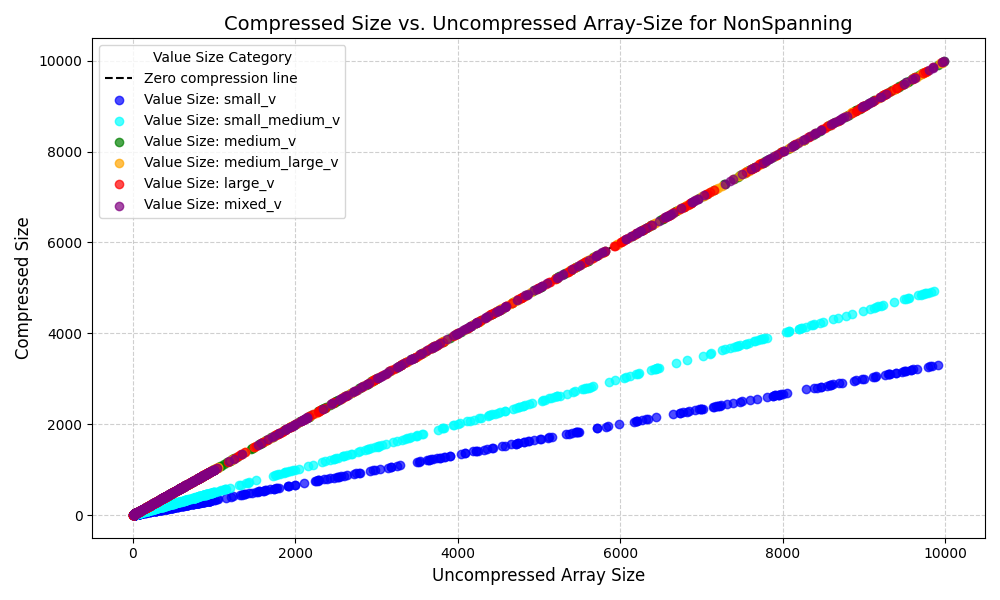
\includegraphics[width=0.8\textwidth]{Grafics/NonSpanning/NonSpanningefficency.png}
		\caption{Compressed array size vs uncompressed array size}
		\label{fig:nonspanning_efficiency}
	\end{figure}
	
	\texttt{Analyse}: We can clearly state that the non spanning compression is only efficent for arrays that contains small values. We have a really good compression for small values (<10bits). At the Array size 10000 for example the compressed array is around 1/3 smaller than the original array. The result is still good for values up to 14 bits. But over this, the compression rate is 0 and superposes the zero compression line equally for the mixed variables arrays.  
	
	\paragraph{The compress method}
	\begin{figure}[H]% =
		\centering
		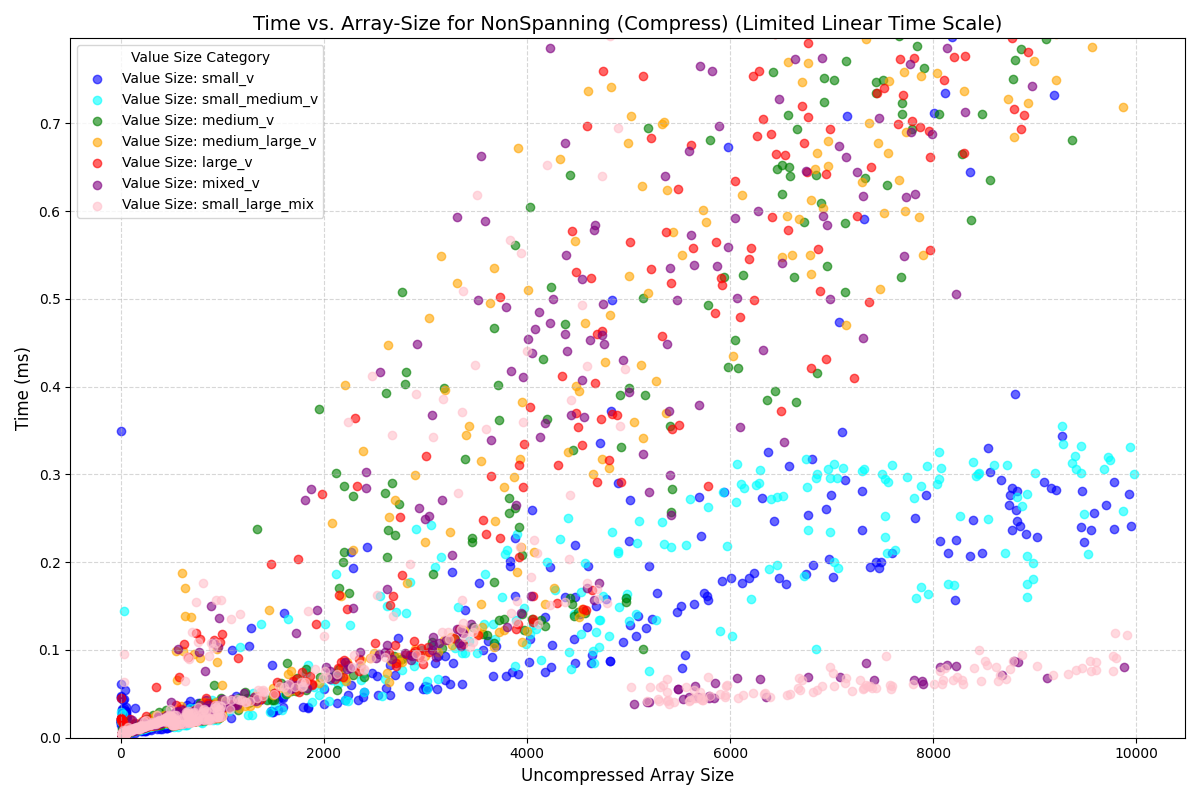
\includegraphics[width=0.8\textwidth]{Grafics/NonSpanning/NonSpanningCompressTimevsSize.png}
		\caption{Non Spanning Compress method: time vs array size}
		\label{fig:4}
		
	\end{figure}
	\begin{figure}[H]% =
		\centering
		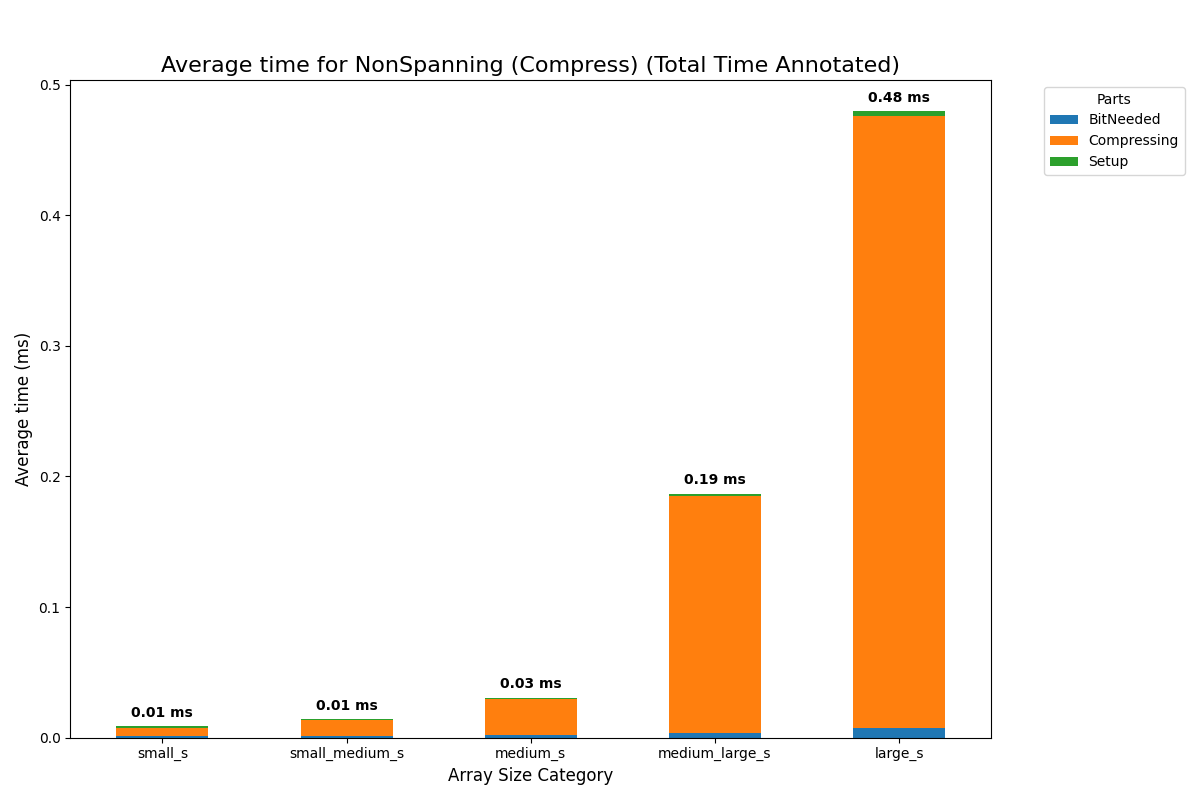
\includegraphics[width=0.8\textwidth]{Grafics/NonSpanning/NonSpanningCompressTime.png}
		\caption{Non Spanning Compress method: avg time vs array size}
		\label{fig:5}
	\end{figure}
	
	\begin{figure}[H]% =
		\centering
		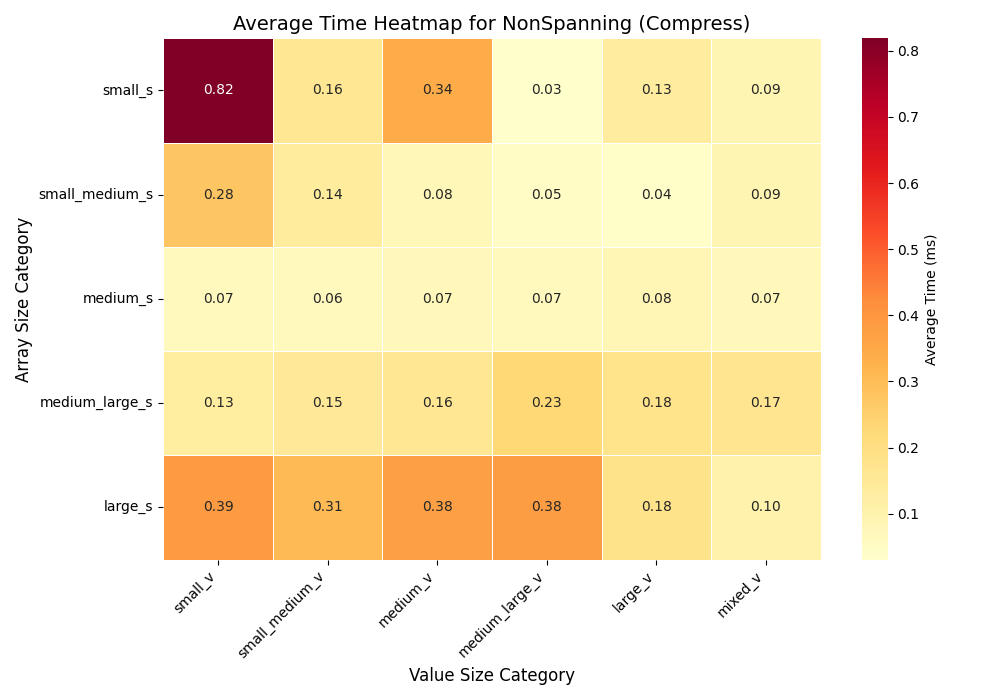
\includegraphics[width=0.8\textwidth]{Grafics/NonSpanning/NonSpanningCompressHeat.png}
		\caption{Non Spanning Compress method: heatmap}
		\label{fig:6}
	\end{figure}
	\texttt{Analyse}: At Figure \ref{fig:4} I observed a strictly increasing runtime across all tested array sizes, confirming that computational time is proportional to data volume. However for small valued arrays this increase is less steep than for the rest  
		\par % 
	
	At Figure \ref{fig:5} I grouped the array sizes and observed the time the different parts take in average to build the average runtime. Interesting is that what we already could observe in the precious figure that the time is increasing other than it may seem it isn't exponential because the possible space for small vsize is a lot less smaller than for large ones
	
	At Figure \ref{fig:6} We can clearly see that the combination of large sized arrays with small values take up to 6-times longer than the other combinations.
	
	\paragraph{The decompression method}
	\begin{figure}[H]% =
		\centering
		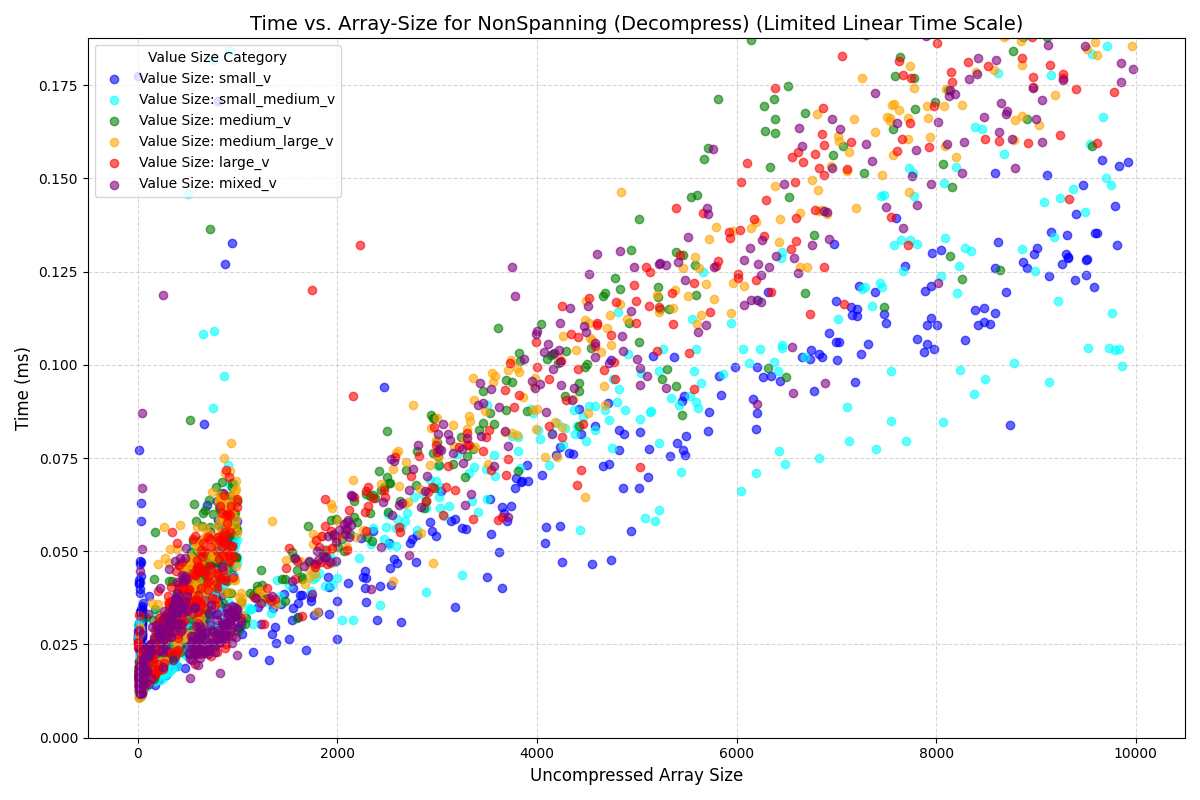
\includegraphics[width=0.8\textwidth]{Grafics/NonSpanning/NonSpanningDecompressTimevsSize.png}
		\caption{Non Spanning Decompress method: time vs array size}
		\label{fig:7}
		
	\end{figure}
	\begin{figure}[H]% =
		\centering
		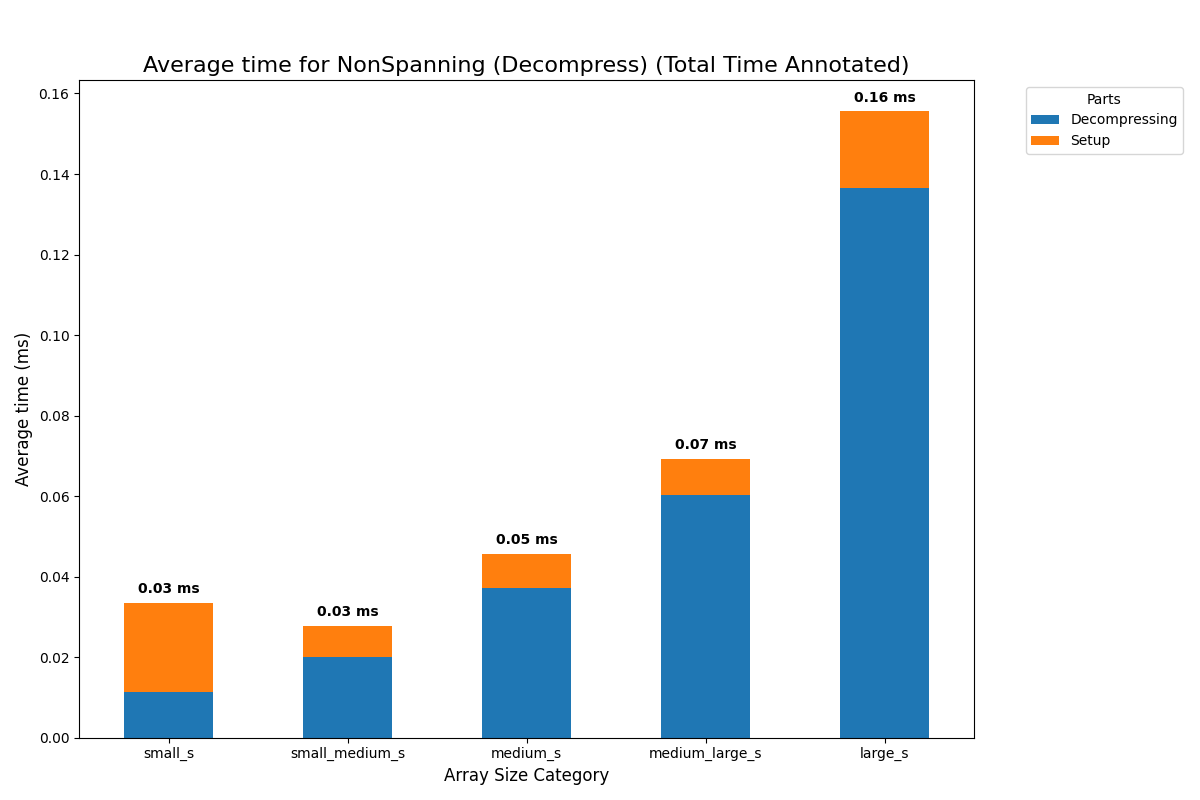
\includegraphics[width=0.8\textwidth]{Grafics/NonSpanning/NonSpanningDecompressTime.png}
		\caption{Non Spanning Decompress method: avg time vs array size}
		\label{fig:8}
	\end{figure}
	
	\begin{figure}[H]% =
		\centering
		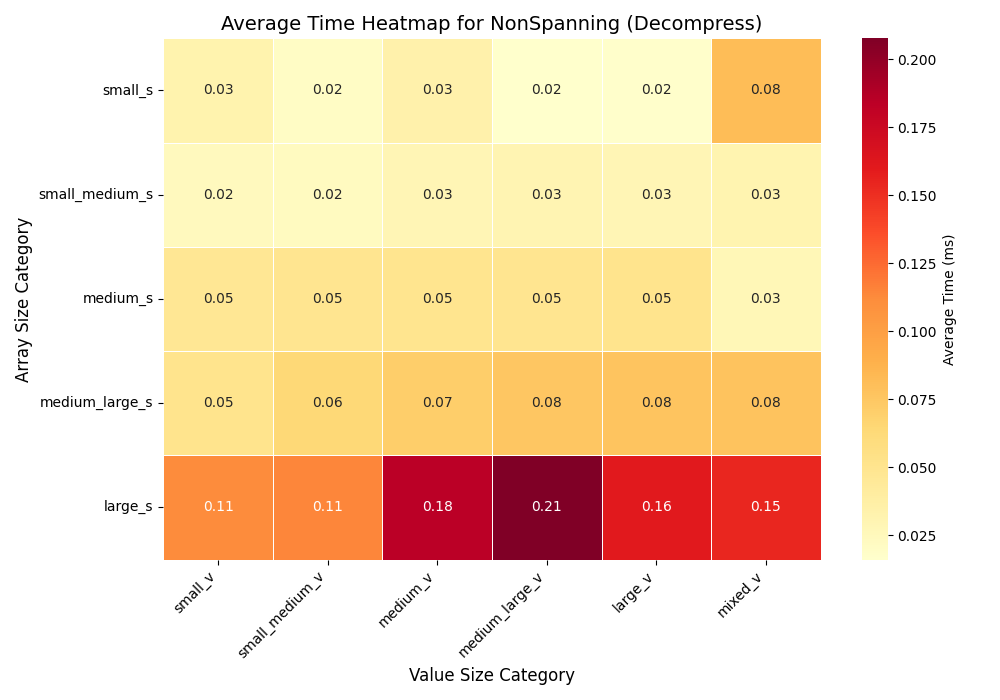
\includegraphics[width=0.8\textwidth]{Grafics/NonSpanning/NonSpanningDecompressHeat.png}
		\caption{Non Spanning Decompress method: heatmap}
		\label{fig:9}
	\end{figure}
	\texttt{Analyse}: At Figure \ref{fig:7} we see a similar evolution as in the compress method. Only we see it is generally faster und that we have for big arrays a large time needed before 5000 array sizes and it inverses afterwards. We can observe this change often at the 5000 mark.
	The Figure \ref{fig:8} shows us that we have an growth with the array size what is confirmed by the anterior figure. Interesting is that the setup for small arrays takes more than half of it's full time.
	The heatmap in Figure \ref{fig:9} jsut confirms our observations in the previous figures.
	  
	\paragraph{The get method}
	\begin{figure}[H]% =
		\centering
		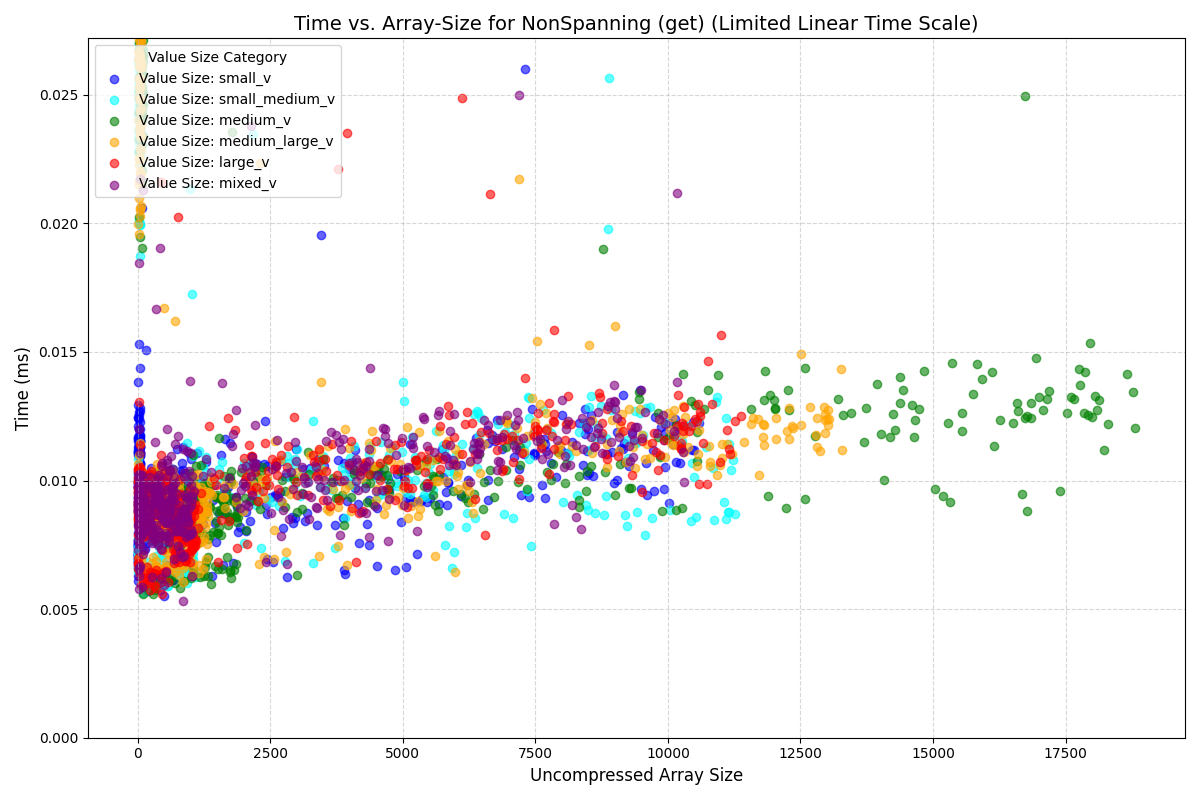
\includegraphics[width=0.8\textwidth]{Grafics/NonSpanning/NonSpanningGetTimevsSize.png}
		\caption{Non Spanning Get method: time vs array size}
		\label{fig:10}
		
	\end{figure}
	
	\begin{figure}[H]% =
		\centering
		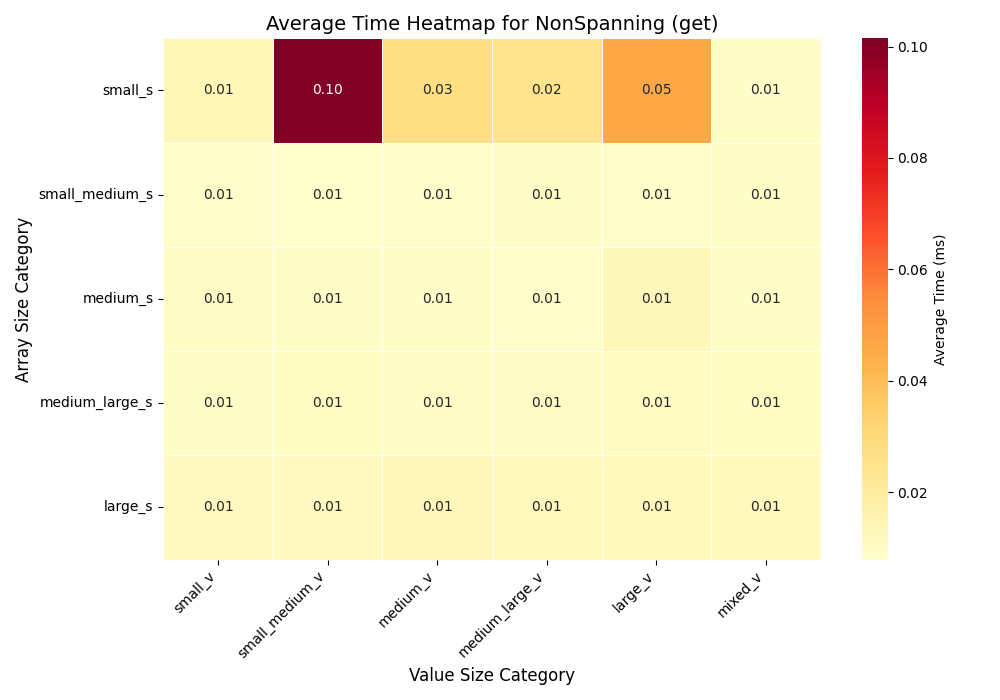
\includegraphics[width=0.8\textwidth]{Grafics/NonSpanning/NonSpanningGetHeat.png}
		\caption{Non Spanning Get method: heatmap}
		\label{fig:11}
	\end{figure}
	\texttt{Analyse}: For the get method it is really easy to analyze we can see clearly in Figure \ref{fig:10} that the time taken is independent of the array size because the average time taken doesn't change significantly this is confirmed by figure \ref{fig:11} where almost every get call is at 0.01ms except for the small sized arrays where it is slightly more.
	
	
	\subsection{Spanning Bit Packing (\texttt{SpanningBP})}
	\label{sec:spanning_bp}
	
	\begin{figure}[h]
		\centering
		\includegraphics[width=0.8\textwidth]{Grafics/spanning.png}
		\caption{Spanning strategy: Example of the architecture of a compressed Integer Array}
		\label{fig:spanning_arch}
	\end{figure}
	
	This implementation focuses purely on maximizing space efficiency. It uses the principle of a continuous bit stream, allowing compressed values to span across the boundary between two adjacent 32-bit integers.
	
	\paragraph{Core Principle: Continuous Bit Stream for Maximum Density}
	\begin{itemize}
		\item \textbf{Maximum Efficiency:} By eliminating all wasted bits caused by word alignment, the compressed array achieves the theoretical minimum size for the given data.
		\item \textbf{High Complexity:} This spatial efficiency comes at the cost of a highly complex implementation, particularly in the bit manipulation logic. Any operation (compress, decompress, or get) must anticipate and correctly handle the conditional scenario where a value is split across two adjacent 32-bit words.
	\end{itemize}
	
	\paragraph{Compression Logic}
	The compression logic for \texttt{SpanningBP} is centered on updating the combined array index (\texttt{result\_cursor}) and the bit offset (\texttt{bit\_cursor}) after processing each value.
	
	\begin{itemize}
		\item Metadata and Spanning Logic: The \texttt{chunk\_size} (5 bits) and the \texttt{nbr\_unused\_bit} (5 bits) are written in the first 10 Bits of the Output-Arrays. The compression loop then checks for boundary crossings for every value. If a value spans, the operation is split into two parts: one part is written to the end of the current word, and the remainder is written to the start of the next word. This is managed by complex bit-masking and shifting.
	\end{itemize}
	
	\paragraph{The \texttt{get} Method (Random Access)}
	Random access is more complex than in the Non-Spanning mode. Access time is still very fast but requires conditional logic to check if the target value is split across two words. If it is split, the value must be reconstructed from two distinct 32-bit words, which increases the computational cost of retrieval compared to the $O(1)$ simplicity of the Non-Spanning method.
	
	\subsection{Analysis of Spanning Bit Packing Strategy}
	\label{sec:strategy_analysis}
	
	
	\paragraph{The compression efficiency}
	
	\begin{figure}[H]% =
		\centering
		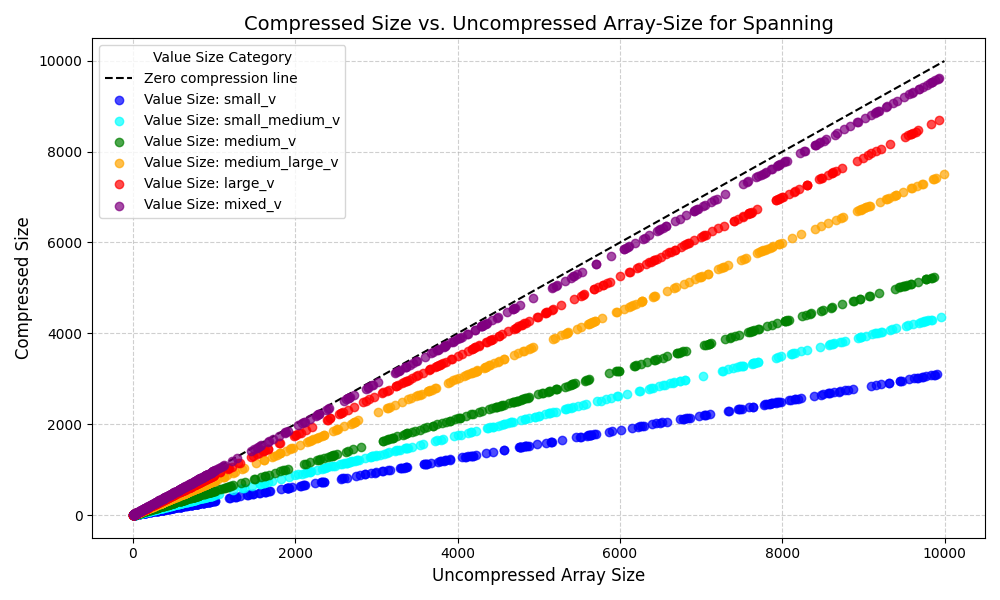
\includegraphics[width=0.8\textwidth]{Grafics/Spanning/Spanningefficency.png}
		\caption{Compressed array size vs uncompressed array size}
		\label{fig:12}
	\end{figure}
	
	\texttt{Analyse}: The Figure \ref{fig:12} shows us really good whenn the Spanning compression method is useful. This is the case when the values in the array are homogeneous and then the smaller these values are the more efficent the compression get. For really small values to a third of its original size and for large values only to 9/10 of its original size. The important thing to state out is that for mixed arrays the compression is marginal. At small array sizes even inexistent.
	
	\paragraph{The compress method}
	\begin{figure}[H]% =
		\centering
		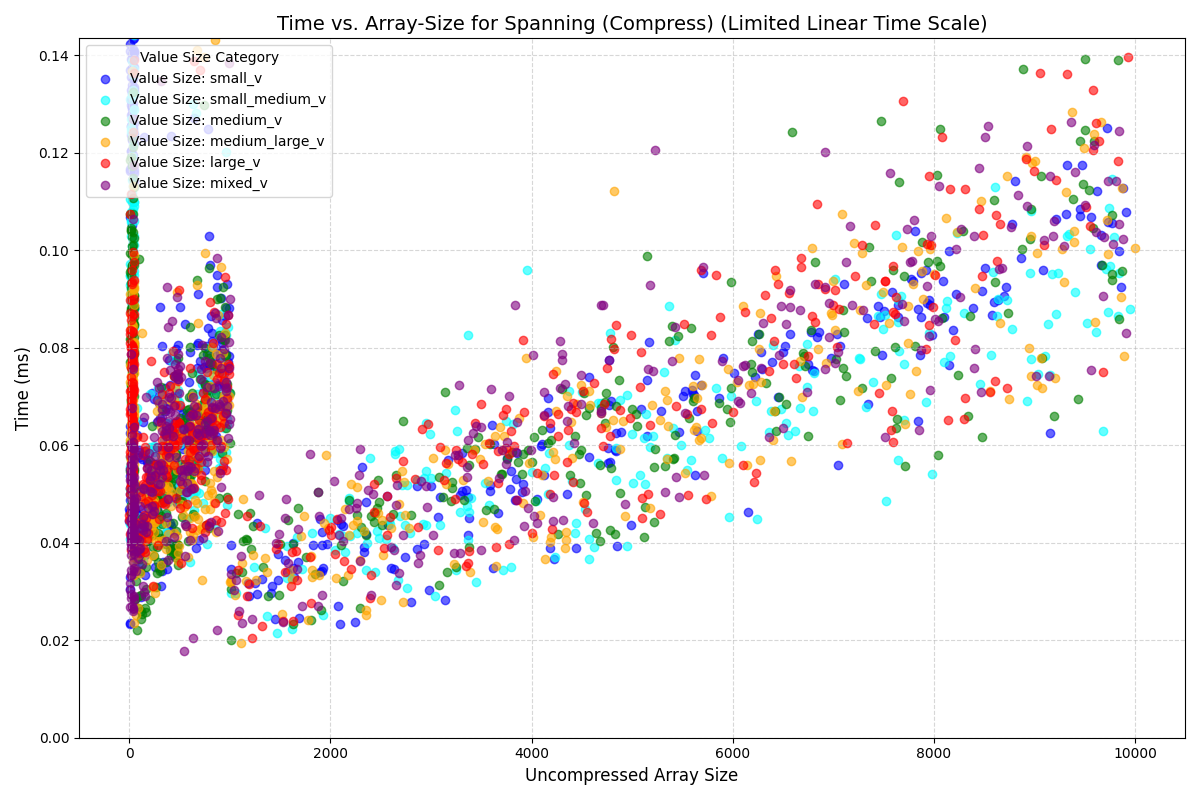
\includegraphics[width=0.8\textwidth]{Grafics/Spanning/SpanningCompressTimevsSize.png}
		\caption{Spanning Compress method: time vs array size}
		\label{fig:13}
		
	\end{figure}
	\begin{figure}[H]% =
		\centering
		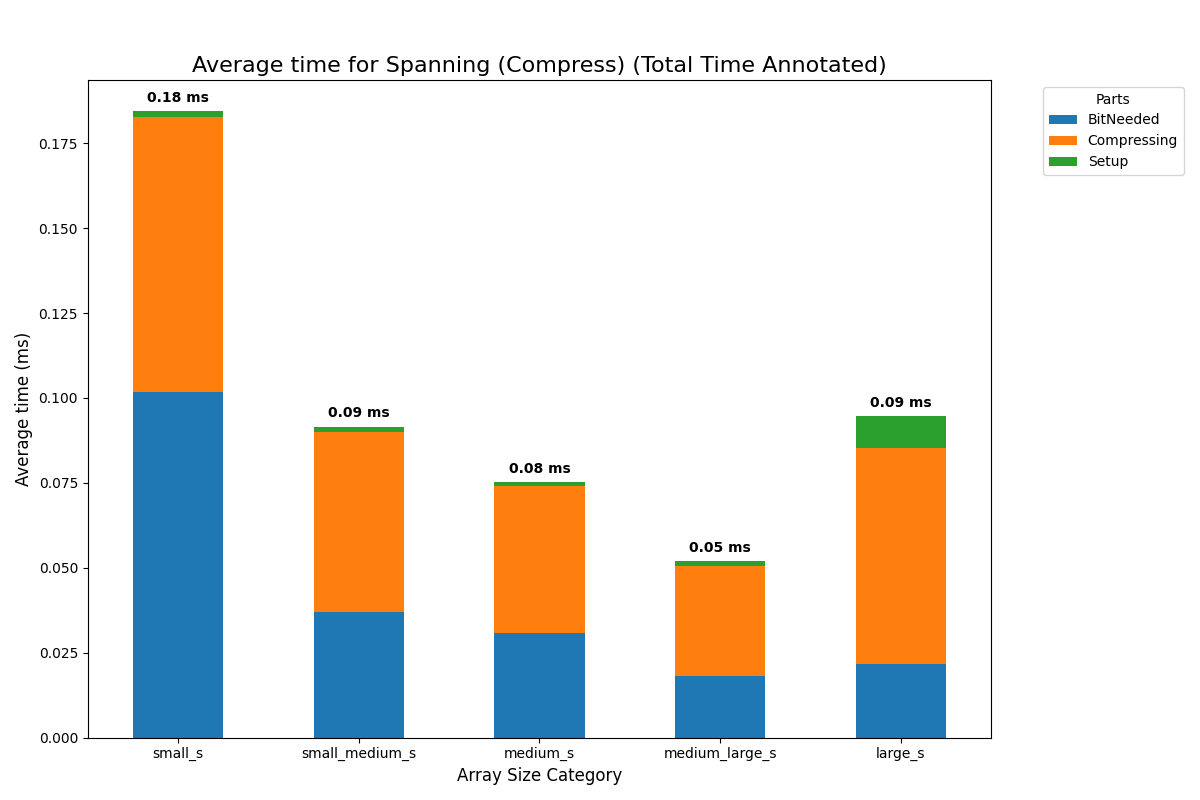
\includegraphics[width=0.8\textwidth]{Grafics/Spanning/SpanningCompressTime.png}
		\caption{Spanning Compress method: avg time vs array size}
		\label{fig:14}
	\end{figure}
	
	\begin{figure}[H]% =
		\centering
		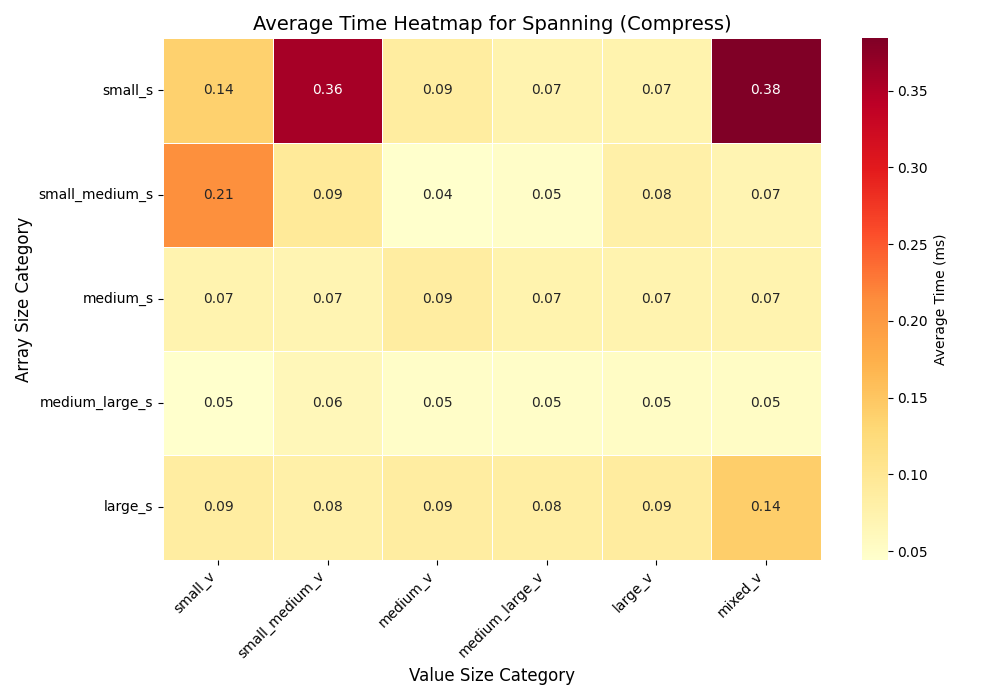
\includegraphics[width=0.8\textwidth]{Grafics/Spanning/SpanningCompressHeat.png}
		\caption{Spanning Compress method: heatmap}
		\label{fig:15}
	\end{figure}
	\texttt{Analyse}: Here at Figure \ref{fig:13} we see a linear growth of the time taken by the compression for a growing array size. Two things fall into the eye: First, for small to medium array sizes this linear growth is steep. Interestingly after 5000 all arrays are treated much faster but again a linear growth wich is less steep than before. 
	
	In Figure \ref{fig:14} we see that the compression time gets higher until a point at the medium large size and then drops again to the same time like the medium arrays. It seems like we have an anomaly at medium large sized arrays, this can be explained with Figure \ref{fig:15} where we see that the higher time taken is high for all of these types of arrays. Which confirms our change at the 5000 sized arrays. 
	\par % 
	
	
	\paragraph{The decompression method}
	\begin{figure}[H]% =
		\centering
		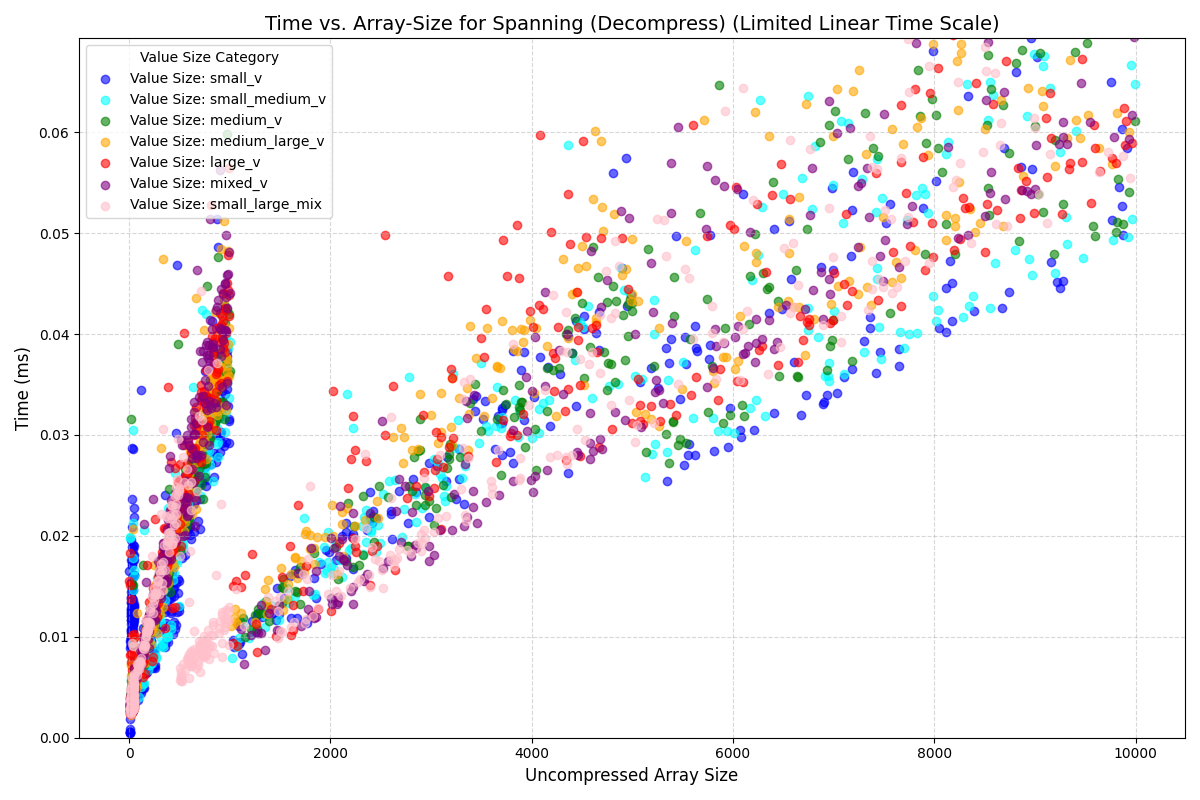
\includegraphics[width=0.8\textwidth]{Grafics/Spanning/SpanningDecompressTimevsSize.png}
		\caption{Spanning Decompress method: time vs array size}
		\label{fig:16}
		
	\end{figure}
	\begin{figure}[H]% =
		\centering
		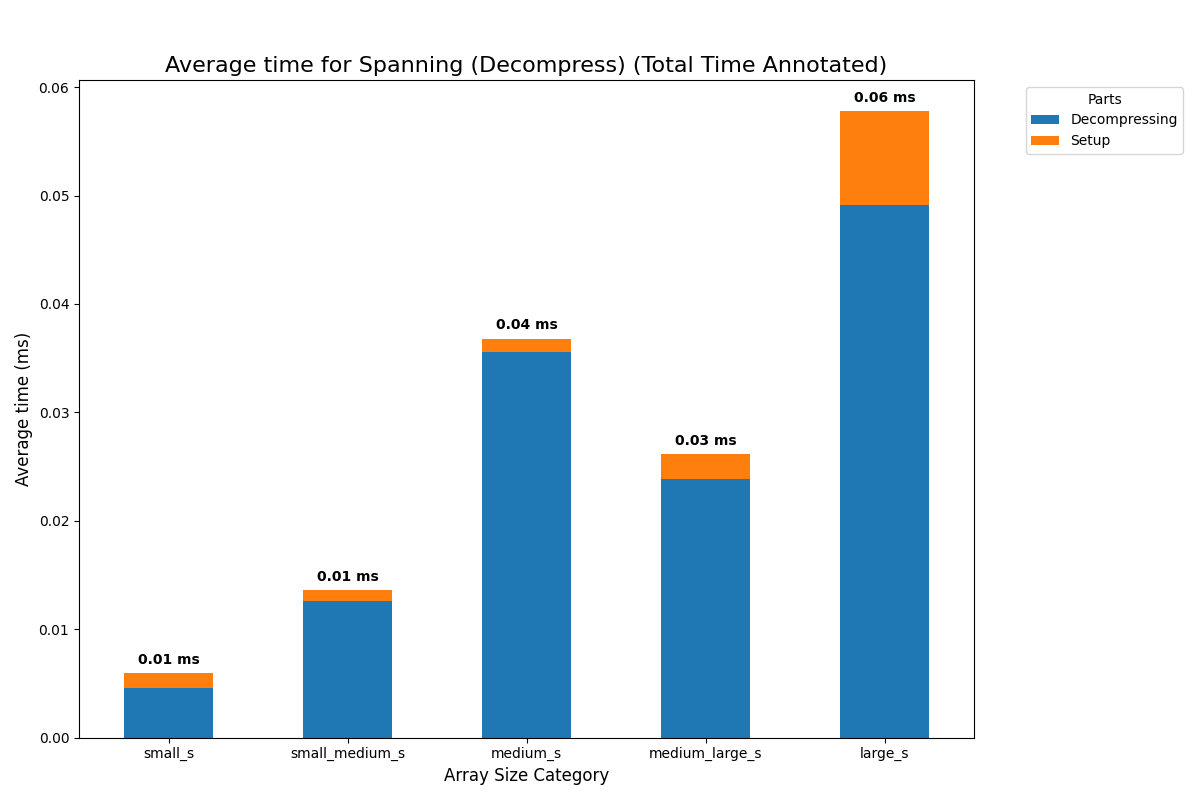
\includegraphics[width=0.8\textwidth]{Grafics/Spanning/SpanningDecompressTime.png}
		\caption{Spanning Decompress method: avg time vs array size}
		\label{fig:17}
	\end{figure}
	
	\begin{figure}[H]% =
		\centering
		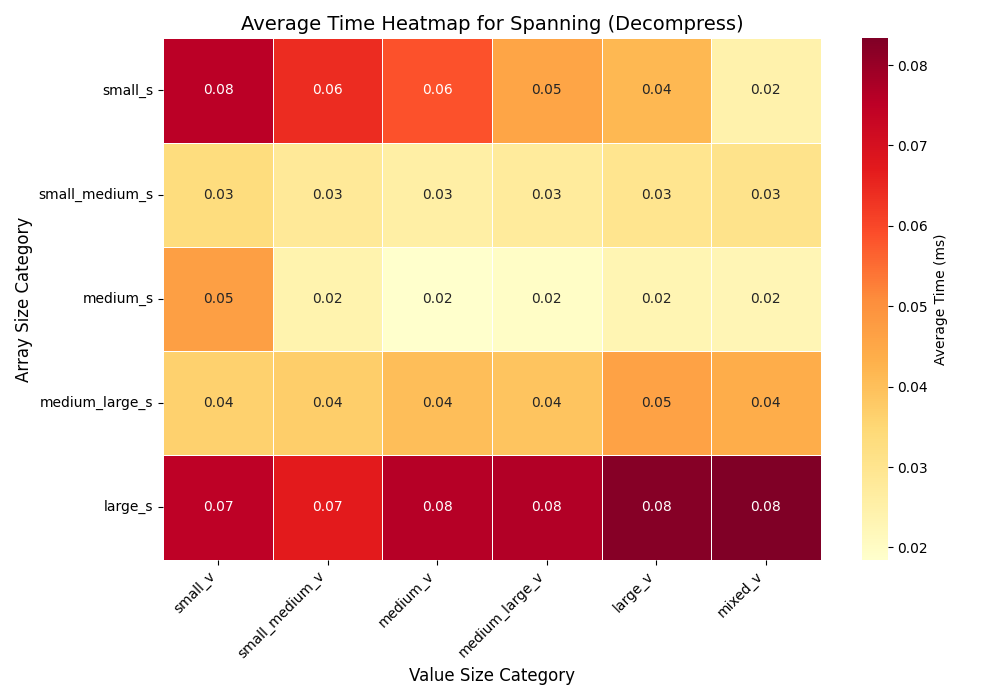
\includegraphics[width=0.8\textwidth]{Grafics/Spanning/SpanningDecompressHeat.png}
		\caption{Spanning Decompress method: heatmap}
		\label{fig:18}
	\end{figure}
	\texttt{Analyse}: The Figure \ref{fig:16} is relatively similar to the Figure \ref{fig:13} in the compress method where we can observe a wider dispersion of the times the bigger the array and anomaly in small array sizes only the turning point is earlier at around 1000.In Figure \ref{fig:17} we have a more or less ninear growth of time xith a little peak at the medium sized arrays. The heatmap at Figure \ref{fig:18} confirms this. But for large arrays we can see that the execution time is the same for all except the small large mix which changes the average.
	
	\paragraph{The get method}
	\begin{figure}[H]% =
		\centering
		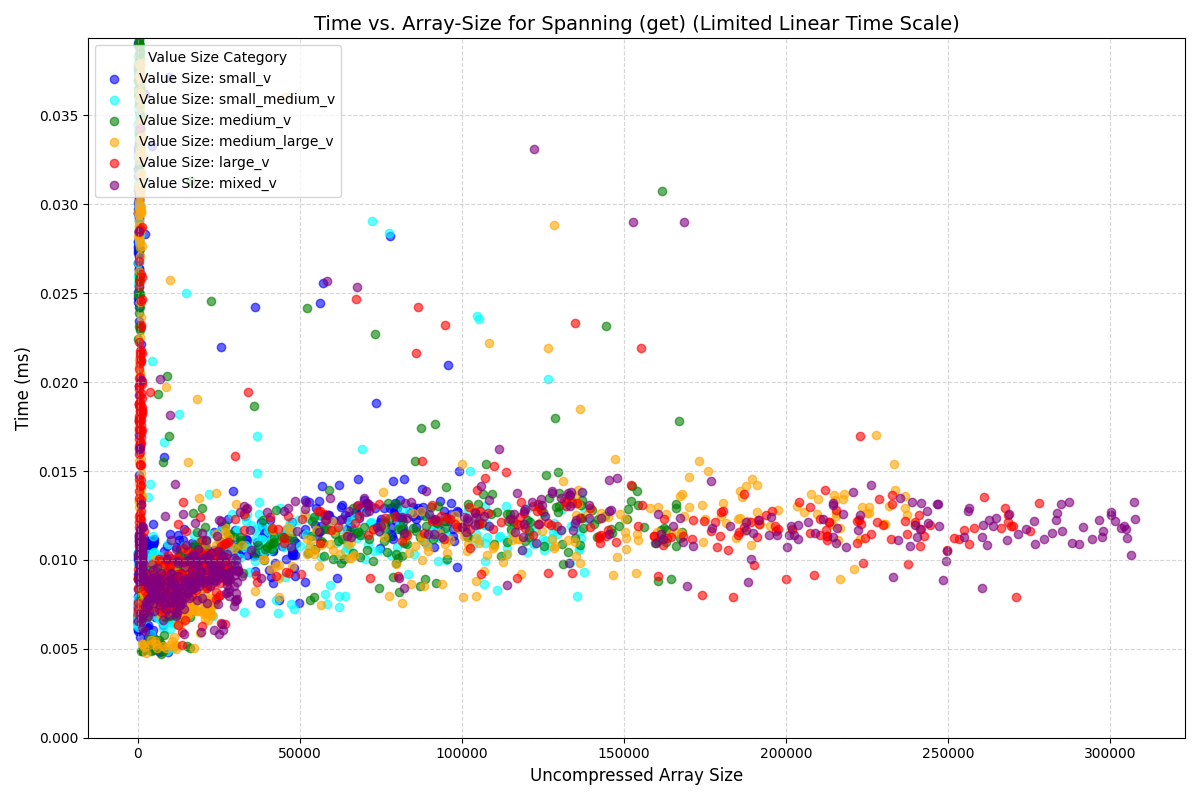
\includegraphics[width=0.8\textwidth]{Grafics/Spanning/SpanningGetTimevsSize.png}
		\caption{Spanning Get method: time vs array size}
		\label{fig:19}
		
	\end{figure}
	
	\begin{figure}[H]% =
		\centering
		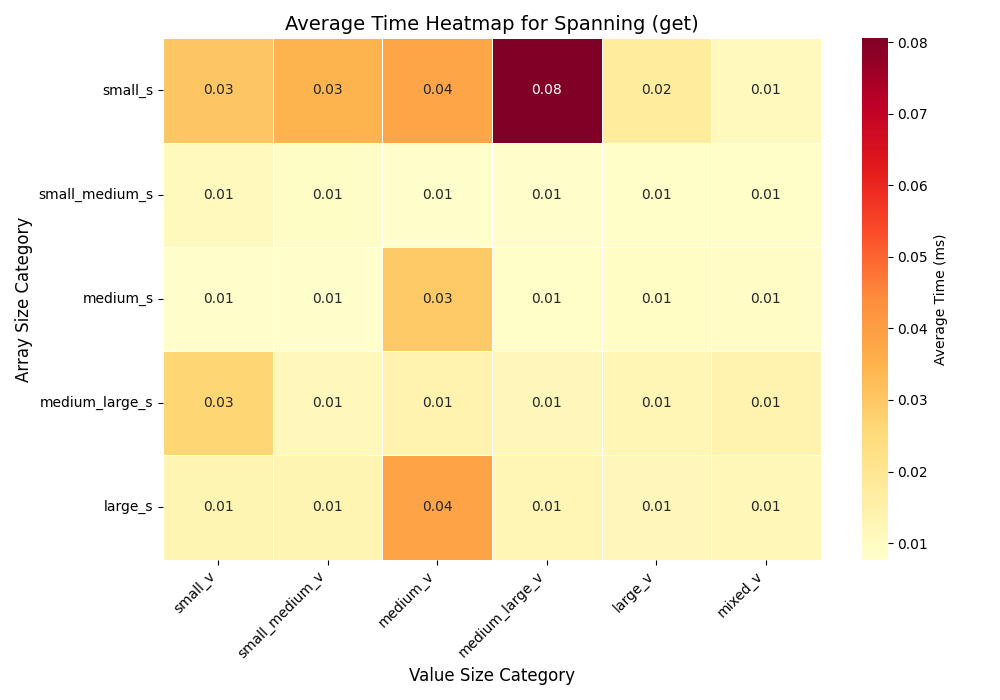
\includegraphics[width=0.8\textwidth]{Grafics/Spanning/SpanningGetHeat.png}
		\caption{Spanning Get method: heatmap}
		\label{fig:20}
	\end{figure}
	\texttt{Analyse}: For the get method we see in Figure \ref{fig:19} that the average time is relatively constant. We have some few exeptions and at really small array sized it can take slightly more time which is confirmed by our heatmap in Figure \ref{fig:20}
	
	\subsection{Overflow Bit Packing (\texttt{OverflowBP})}
	\label{sec:overflow_bp}
	
	\begin{figure}[h]
		\centering
		\includegraphics[width=0.8\textwidth]{Grafics/overflow.png}
		\caption{Overflow strategy: Example of the architecture of a compressed Integer Array}
		\label{fig:overflow_arch}
	\end{figure}
	
	The \texttt{OverflowBP} is a hybrid strategy based on the Spanning mechanism, designed to handle arrays where the majority of values are small but a few outliers exist.
	
	\paragraph{Core Principle: Separating Outliers}
	This method aims to achieve high compression for the majority of data by using a small **optimal chunk size** ($k'$) while still accommodating large outliers:
	\begin{enumerate}
		\item Optimal Size: We calculate the smallest $k'$ that covers most values.
		\item Main Stream: Normal values are packed into the main stream using $k'$ bits. An extra marker bit (0) is used to indicate a normal value.
		\item Overflow Area: Values that exceed the $k'$ capacity are moved to a separate Overflow Area. In the main stream, a marker bit (1) and an index pointing to the value's full 32-bit location in the Overflow Area are stored.
	\end{enumerate}
	
\paragraph{The \texttt{compress} Method}
The compression process is the most complex of the three strategies, integrating the optimal size calculation, Elias Gamma encoding, and the spanning logic:

\begin{itemize}
	\item \textbf{Metadata and Elias Gamma Encoding:} Besides the 10 bits for \texttt{chunk\_size} and \texttt{unused\_bits}, the metadata includes the size of the Overflow Area, which is encoded using the Elias Gamma scheme \ref{elias}. This variable-length encoding provides a compact way to store the overflow count, minimizing overhead.
	\item \textbf{Dual Stream Packing:} The loop iterates over the original data. If a value overflows, a marker bit '1' is written to the main stream, the original value is stored in the Overflow Area, and the index of that storage location is written back into the main stream using the small \texttt{chunk\_size}. If the value is normal, a marker bit '0' is written, followed by the value itself.
	\item \textbf{Spanning Logic:} The writing of both the marker bit (1 bit) and the value/index chunk (\texttt{chunk\_size} bits) must adhere to the Spanning logic to ensure no bit is wasted, treating the marker bit and the value/index chunk as a single $ (\texttt{chunk\_size} + 1) $-bit entity.
\end{itemize}

\paragraph{The \texttt{decompress} and \texttt{get} Methods}
Decompression and random access must meticulously follow the structure defined by the Overflow strategy:

\begin{enumerate}
	\item \textbf{Metadata Decoding:} The method first reads the \texttt{chunk\_size} and \texttt{unused\_bits}, and then uses the \texttt{decodeEliasGamma} helper function to determine the size of the Overflow Area.
	\item \textbf{Marker Check:} For each value, the method first checks the marker bit:
	\begin{itemize}
		\item If the marker is \texttt{0}, the subsequent \texttt{chunk\_size} bits are extracted from the main stream, adhering to the spanning logic, and this is the final value.
		\item If the marker is \texttt{1}, the subsequent \texttt{chunk\_size} bits are extracted from the main stream (this value is the overflow index). This index is then used to look up the original, full 32-bit value in the Overflow Area.
	\end{itemize}
	\item \textbf{Random Access (\texttt{get}):} The \texttt{get} method is significantly more complex than in \texttt{NonSpanningBP} because it must first calculate the exact bit position using the variable-length Elias Gamma metadata and the $ (\texttt{chunk\_size} + 1) $ entity size, and then perform the marker check and potential spanning extraction to retrieve the final result.
\end{enumerate}

	
	\subsection{Analysis of Overflow Bit Packing Strategy}
	
	
	\paragraph{The compression efficiency}
	
	\begin{figure}[H]% =
		\centering
		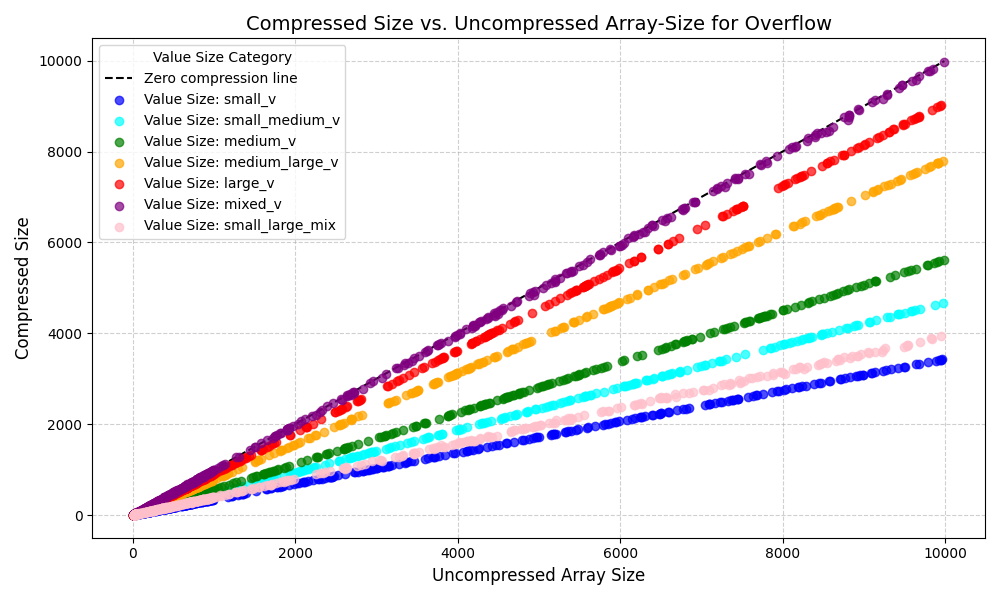
\includegraphics[width=0.8\textwidth]{Grafics/Overflow/Overflowefficency.png}
		\caption{Compressed array size vs uncompressed array size}
		\label{fig:21}
	\end{figure}
	\texttt{Analyse}: The Figure \ref{fig:21} shows us a Figure really similar to the Figure \ref{fig:12} . The only but important difference is that for small\_large\_mix which took at the spanning compression as much space as an large valued array. But here it takes just a little more than a a small array. This shows that the Overflow strategy is effective but needs a non homogeneous array to have an impact.  
	
	\paragraph{The compress method}
	\begin{figure}[H]% =
		\centering
		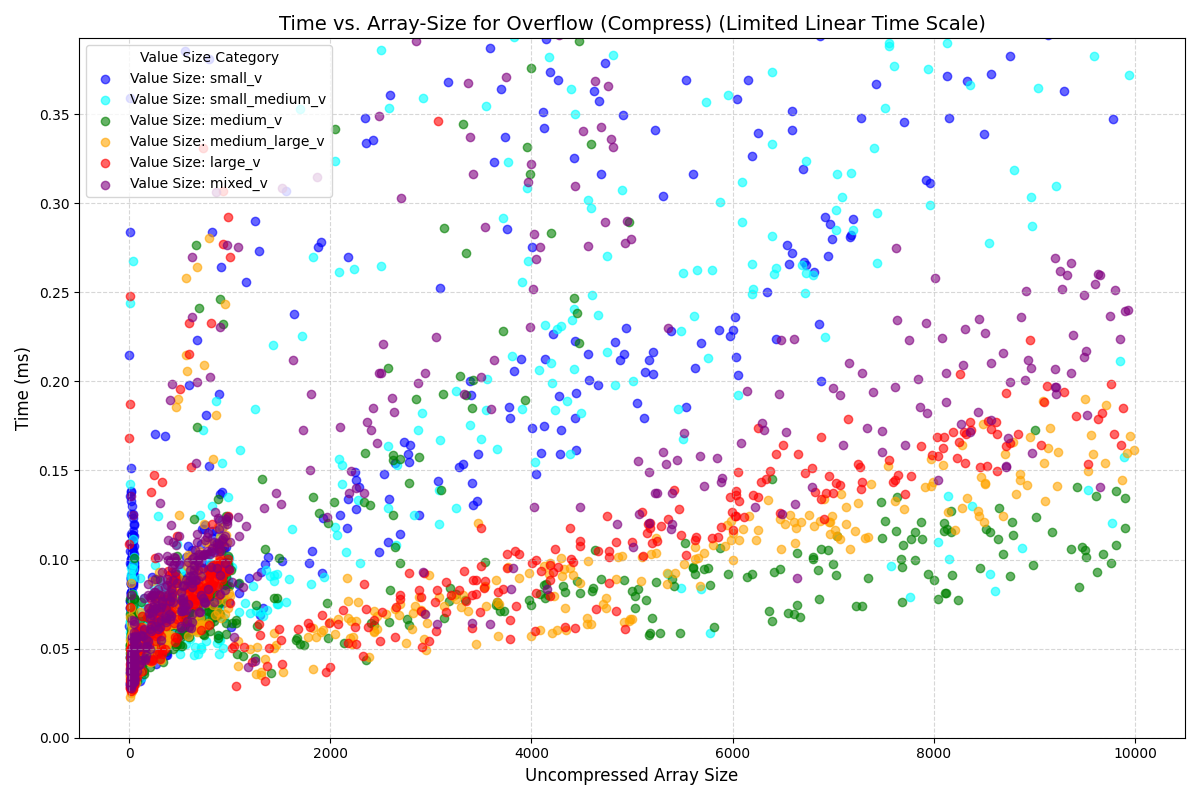
\includegraphics[width=0.8\textwidth]{Grafics/Overflow/OverflowCompressTimevsSize.png}
		\caption{Overflow Compress method: time vs array size}
		\label{fig:23}
		
	\end{figure}
	\begin{figure}[H]% =
		\centering
		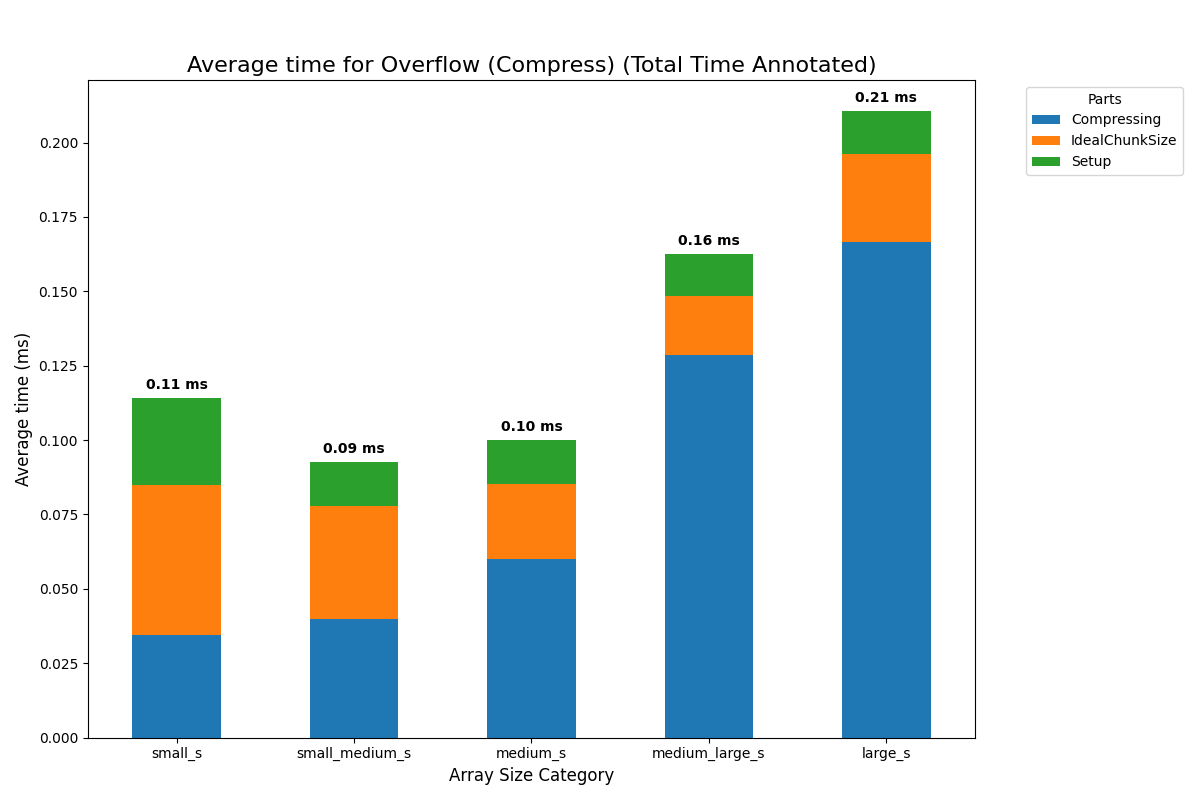
\includegraphics[width=0.8\textwidth]{Grafics/Overflow/OverflowCompressTime.png}
		\caption{Overflow Compress method: avg time vs array size}
		\label{fig:24}
	\end{figure}
	
	\begin{figure}[H]% =
		\centering
		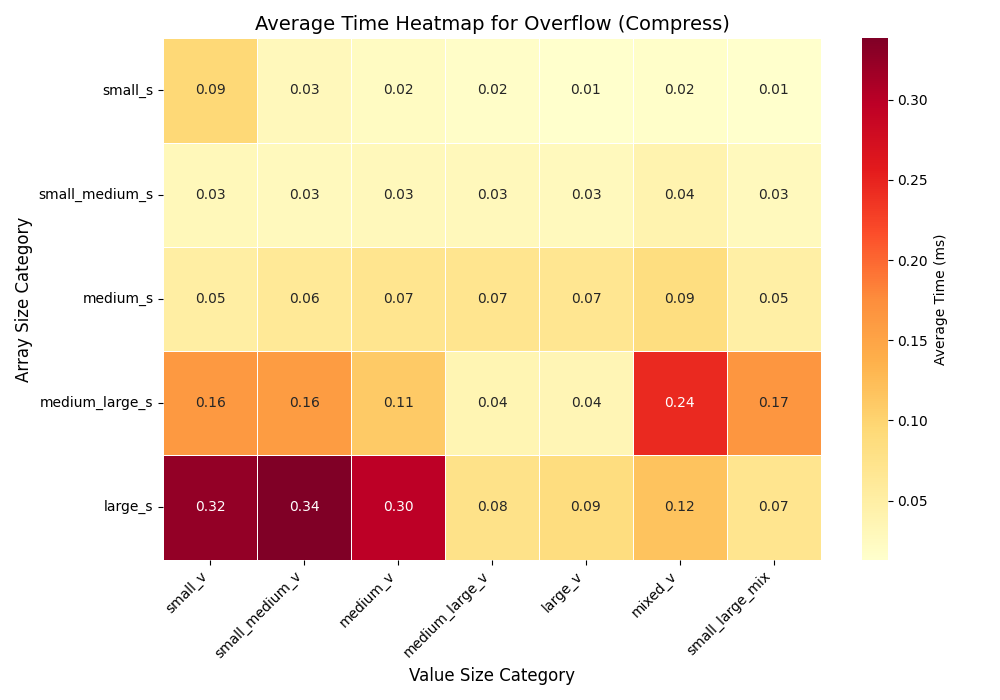
\includegraphics[width=0.8\textwidth]{Grafics/Overflow/OverflowCompressHeat.png}
		\caption{Overflow Compress method: heat map}
		\label{fig:25}
	\end{figure}
	\texttt{Analyse}: The Figure \ref{fig:23} shows us for the most types of arrays a linear growth of time. But different to the other strategies we can see a separation between the value types wich indicates that those also have an influence on the execution time. We have equally a linear growth in Figure\ref{fig:24} the minima is now how we can see in Figure \ref{fig:25} placed more in the large value and small size arrays with a maxima at the large array small value side 
	\par % 
	
	
	\paragraph{The decompression method}
	\begin{figure}[H]% =
		\centering
		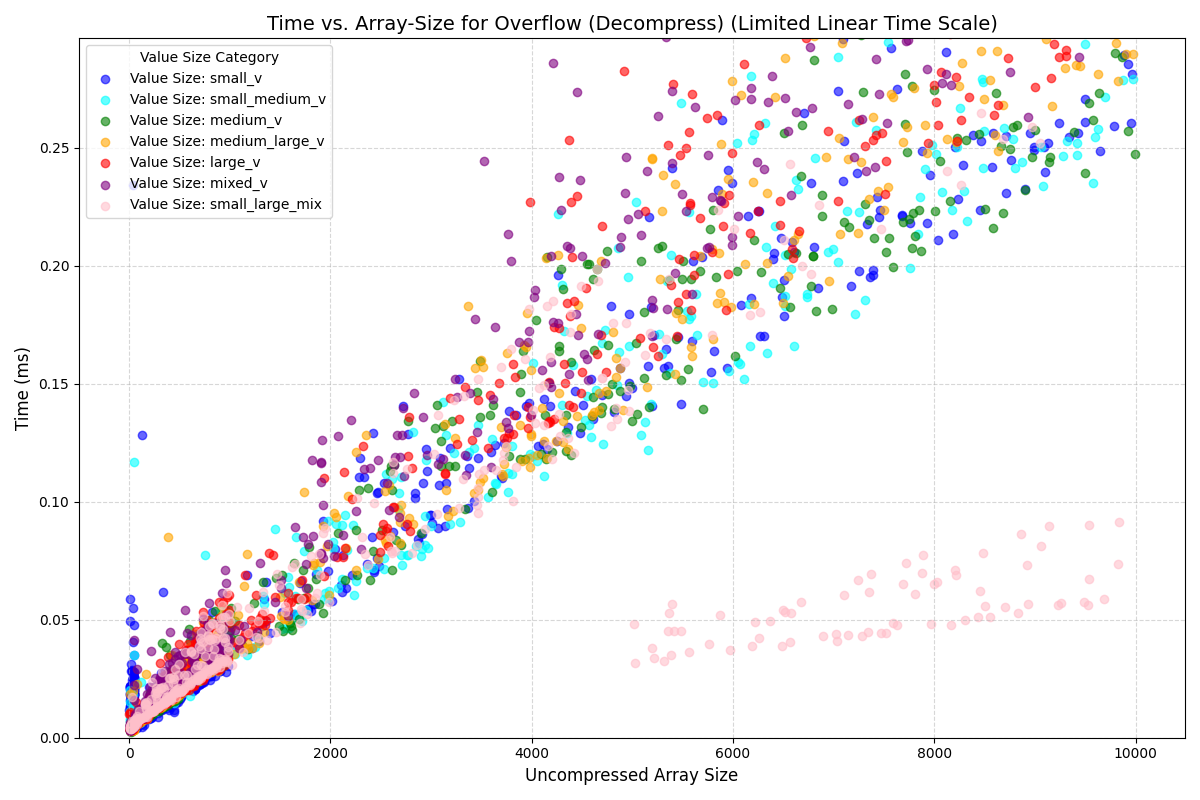
\includegraphics[width=0.8\textwidth]{Grafics/Overflow/OverflowDecompressTimevsSize.png}
		\caption{Overflow Decompress method: time vs array size}
		\label{fig:26}
		
	\end{figure}
	\begin{figure}[H]% =
		\centering
		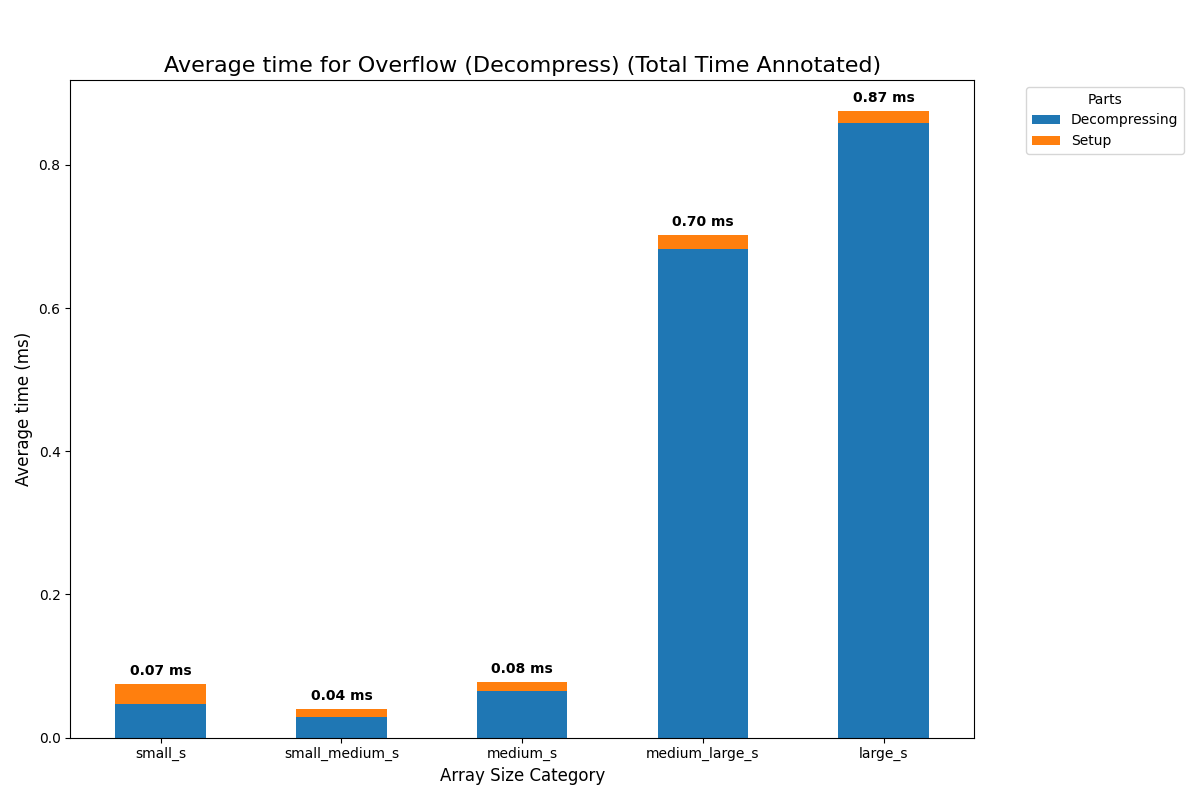
\includegraphics[width=0.8\textwidth]{Grafics/Overflow/OverflowDecompressTime.png}
		\caption{Overflow Decompress method: avg time vs array size}
		\label{fig:27}
	\end{figure}
	
	\begin{figure}[H]% =
		\centering
		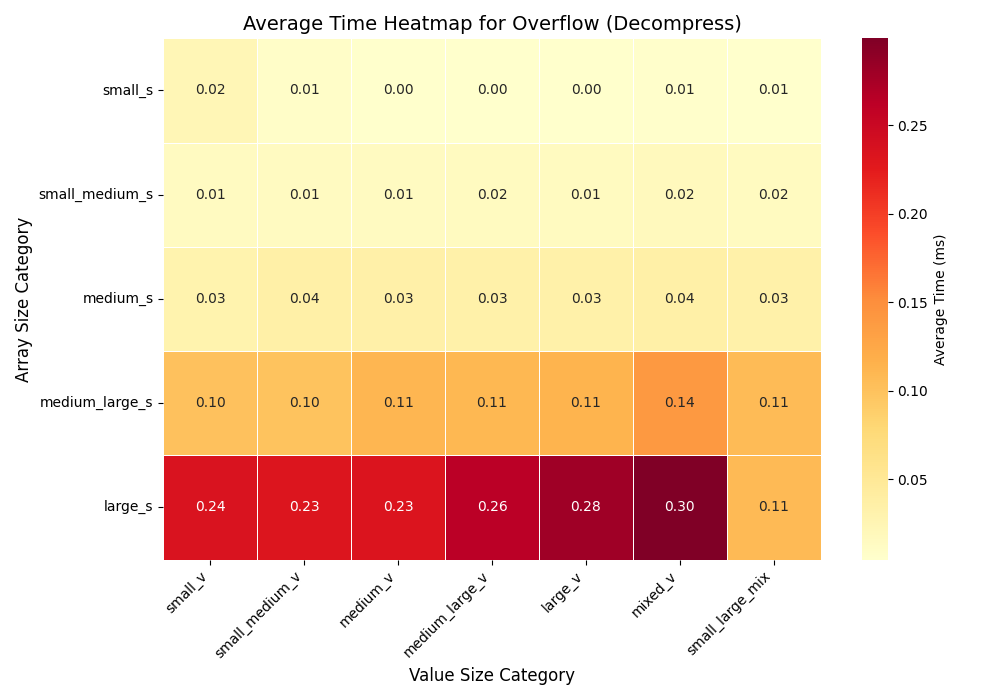
\includegraphics[width=0.8\textwidth]{Grafics/Overflow/OverflowDecompressHeat.png}
		\caption{Overflow Decompress method: heatmap}
		\label{fig:28}
	\end{figure}
	\texttt{Analyse}: The decompression method shows in Figure \ref{fig:26} a steep growth of time with growing arrays where the dispersion of the time off the average time gets bigger the bigger the array. With the exception after 5000 array size for the small\_large mixed values which get really effective. Figure \ref{fig:27} shows  an linear growth of the average time taken. The heat map \ref{fig:28} shows that especially for large arrays it takes up to 10 times as much time as the category beneath.
	
	\paragraph{The get method}
	\begin{figure}[H]% =
		\centering
		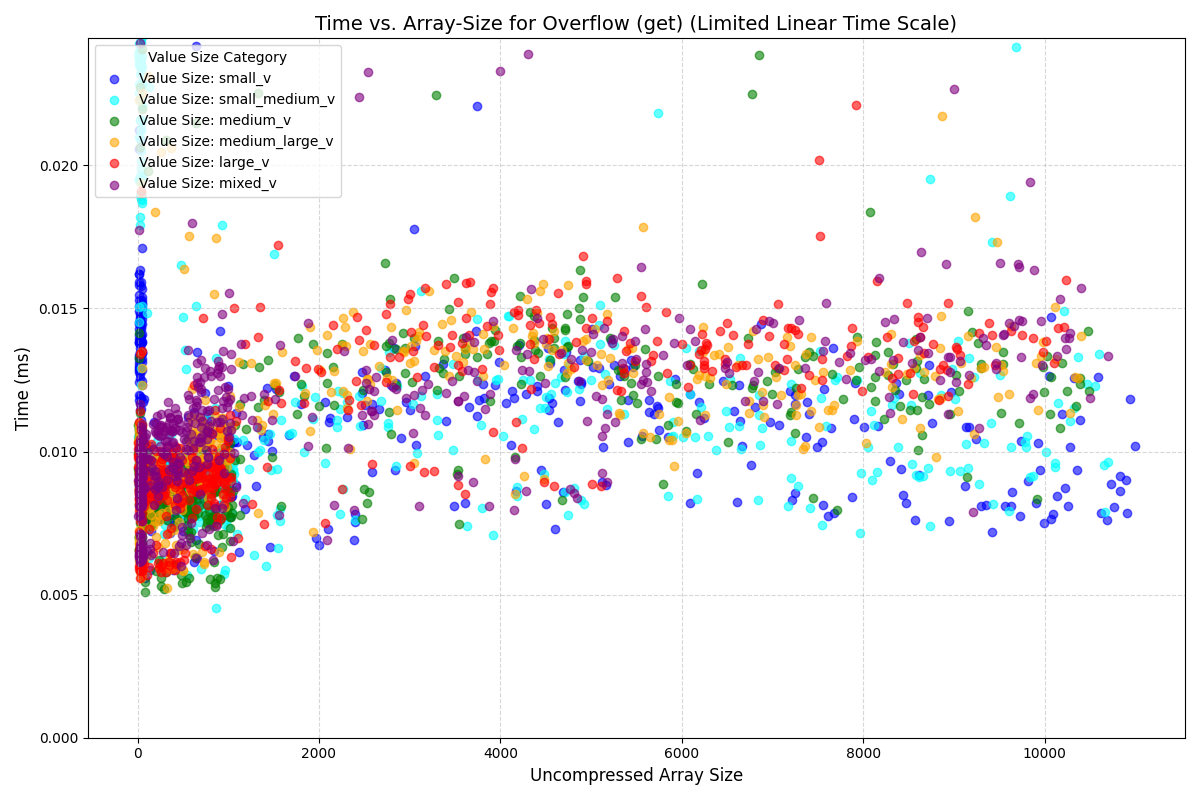
\includegraphics[width=0.8\textwidth]{Grafics/Overflow/OverflowGetTimevsSize.png}
		\caption{Spanning Get method: time vs array size}
		\label{fig:29}
		
	\end{figure}
	
	\begin{figure}[H]% =
		\centering
		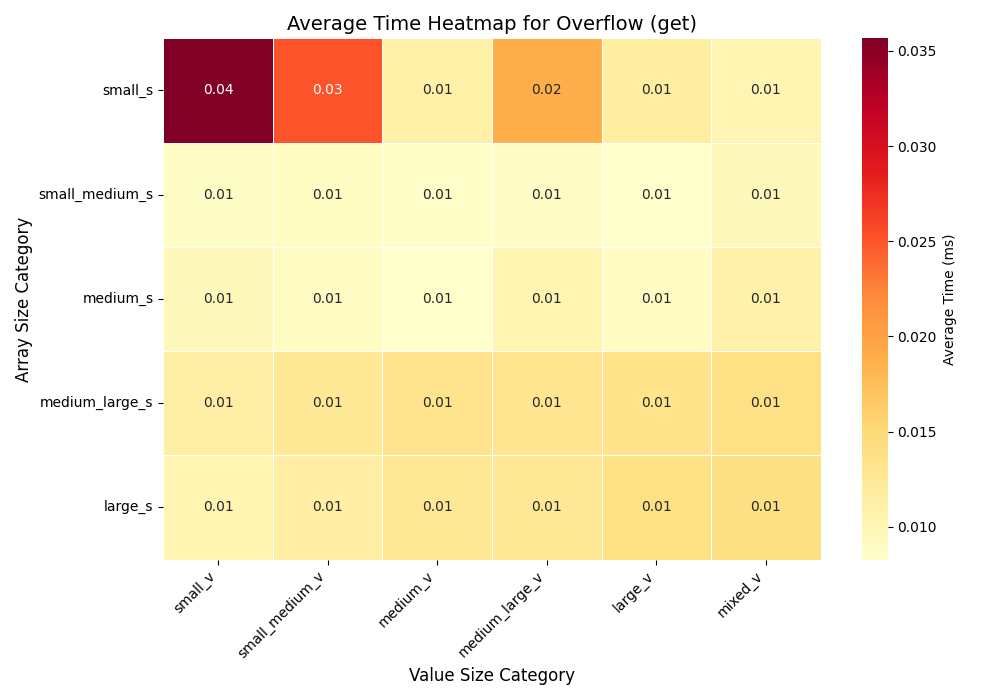
\includegraphics[width=0.8\textwidth]{Grafics/Overflow/OverflowGetHeat.png}
		\caption{Spanning Get method: heatmap}
		\label{fig:30}
	\end{figure}
	\texttt{Analyse}: The get method stays relatively solid with O(n) as complexity. We can observe like in the other strategys a high average time for small arrays.
	
	
	\section{Comparison of the Compression Strategies}
	\begin{figure}[H]% =
		\centering
		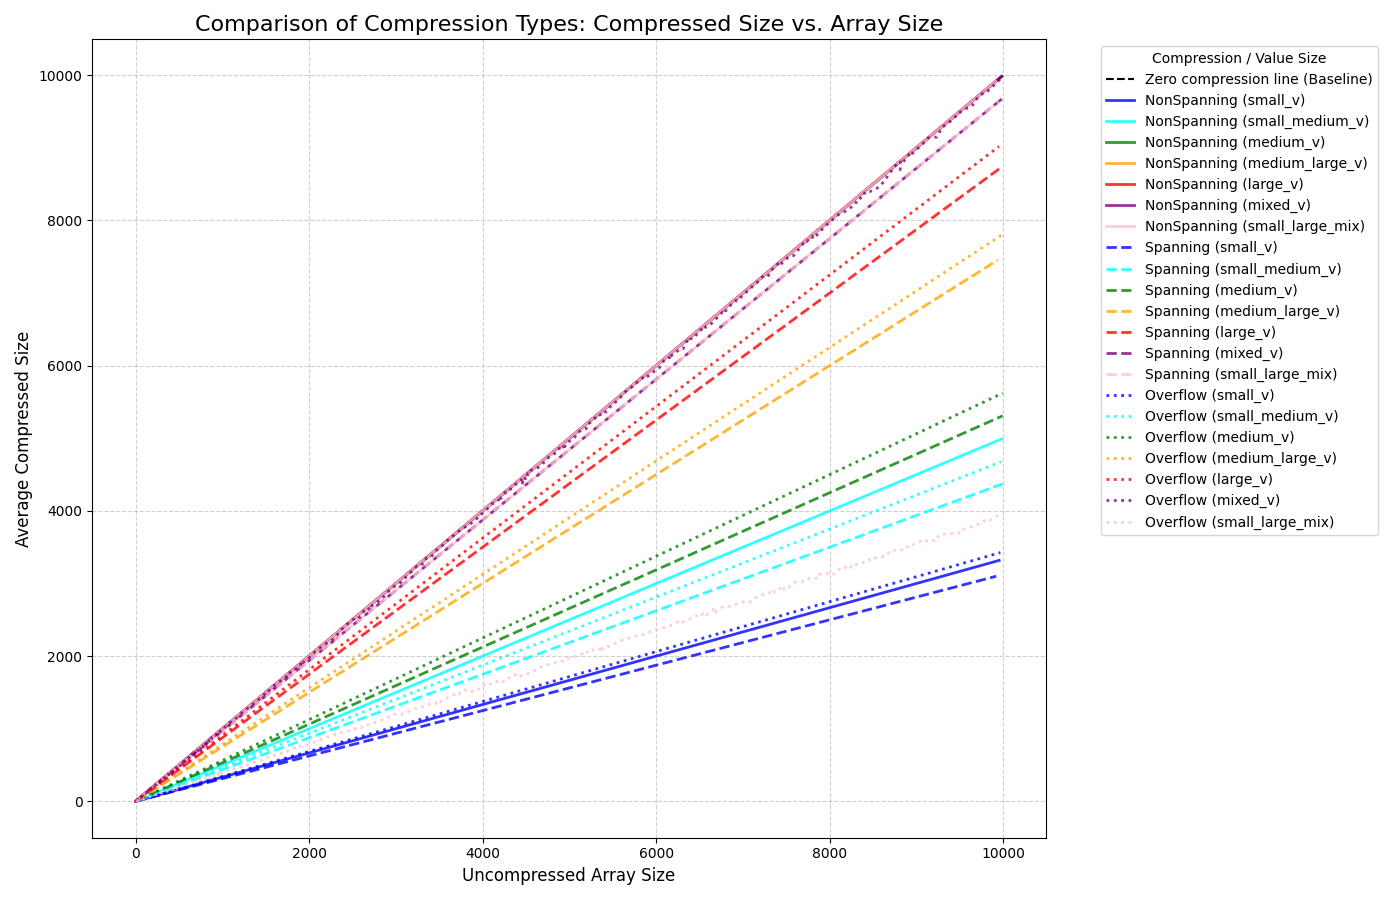
\includegraphics[width=0.8\textwidth]{Grafics/Compare/Comparingcompression.png}
		\caption{Comparison of compression effectiveness}
		\label{fig:31}
	\end{figure}
	\begin{figure}[H]% =
		\centering
		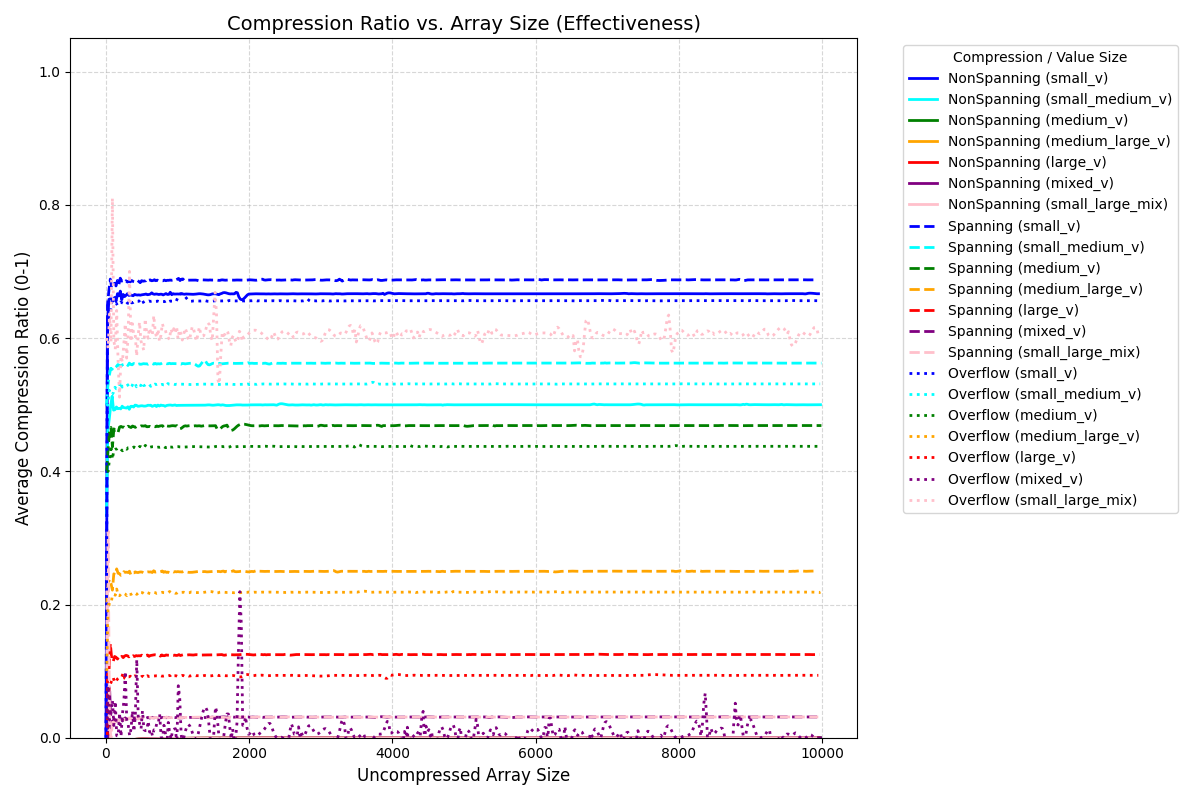
\includegraphics[width=0.8\textwidth]{Grafics/Compare/ComparingEffectivenesscompression.png}
		\caption{Comparison of compression effectiveness}
		\label{fig:32}
	\end{figure}
	\texttt{Analyse}: Figure \ref{fig:31} and \ref{fig:32} show us what we already analyzed in the graphs for each compression strategy. What we can observe is that in our test cases  We can observe almost for each category the same pattern: The nonSpanning strategy is the least effective and the spanning in our test cases the most effective because we have many homogenous arrays. The overflow strategy is always in between both but can at some cases be more effective. This is the case for arrays with many small values and very fey big ones. where it gets really effective
	\begin{figure}[H]% =
		\centering
		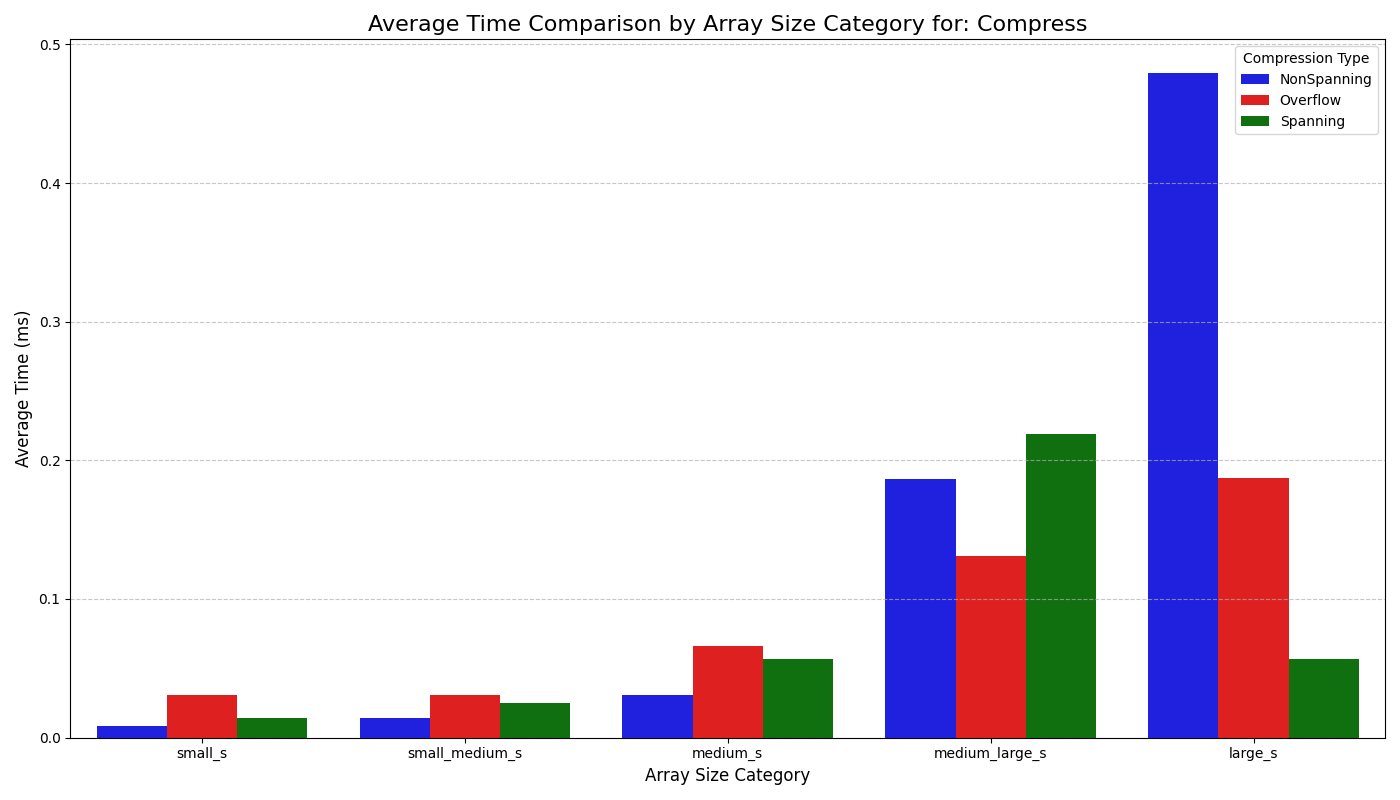
\includegraphics[width=0.8\textwidth]{Grafics/Compare/ComparingCompressTime.png}
		\caption{Comparison of compression effectiveness}
		\label{fig:33}
		\end{figure}
	\begin{figure}[H]% =
		\centering
		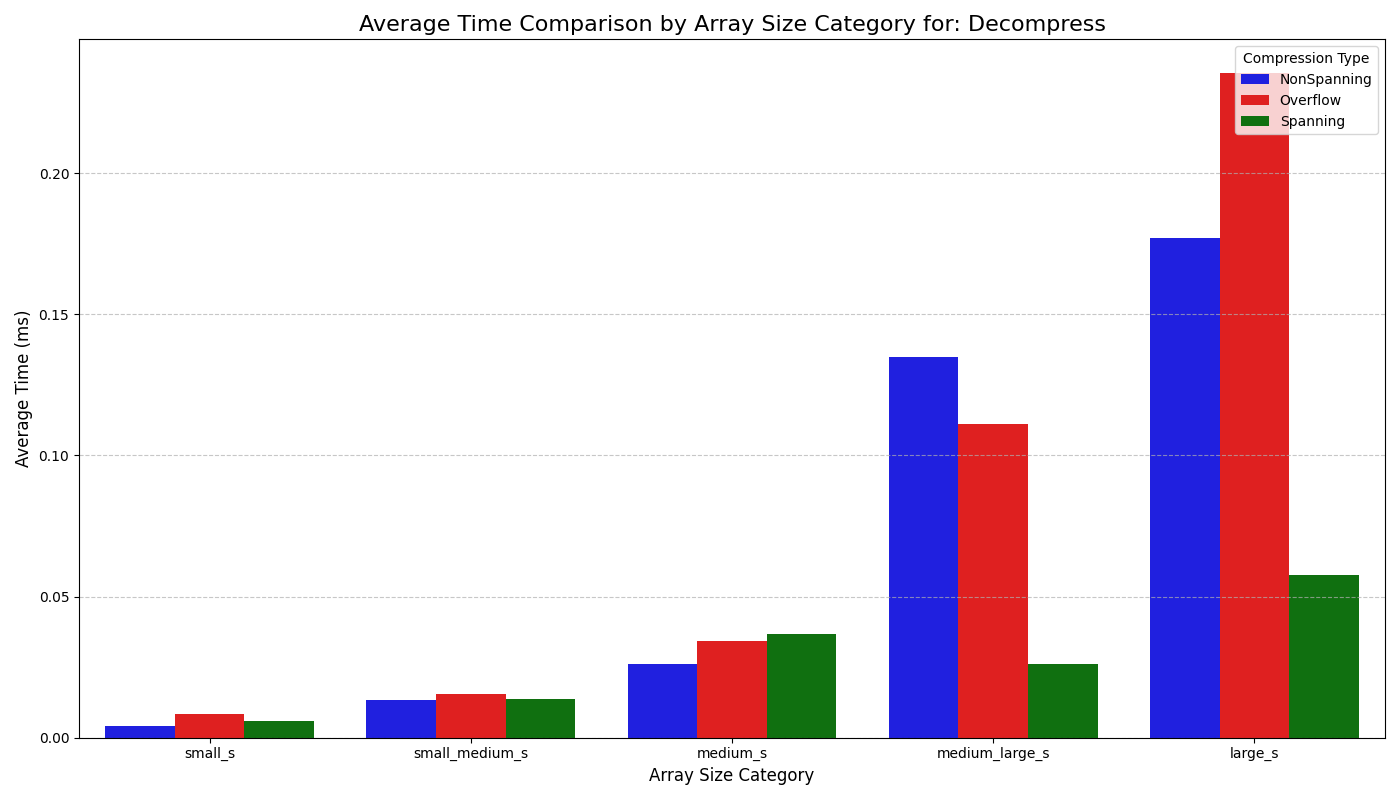
\includegraphics[width=0.8\textwidth]{Grafics/Compare/ComparingDecompressTime.png}
		\caption{Comparison of compression effectiveness}
		\label{fig:34}
	\end{figure}
	\texttt{Analyse}: Analysing the time each compression strategy takes to compress \ref{fig:33} is interesting because for the spanning strategy the time taken is getting shorter with the array size and gets bigger only at really large arrays and its the opposite for the other two compression methods. For the decompression method really interesting is that the Overflow method for really big arrays is more than 4 times higher than the spanning strategies at the same arrays. Interesting is that the non spanning strategy takes for the compression more time at large arrays which shouldnt be the case because it is the less complicated to calculate.
	
	\section{Handling Negative Integers (Proposition)}
	
	\subsection{Adaptation using a Dedicated Sign Bit}
	
	The three compression strategies discussed so far (Non-Spanning, Spanning, Overflow) implicitly assume positive, unsigned integers, as Bit Packing fundamentally operates on the magnitude (the required bit size, $k$). To extend this framework to support negative numbers—i.e., standard Java \texttt{int} values—I propose a simple, robust adaptation using a dedicated sign bit.
	
	\paragraph{Proposed Mechanism: Sign Bit Overhead}
	For every $k$-bit compressed integer, we allocate one additional bit ($S$) dedicated solely to storing the sign information, resulting in a total size of $(k+1)$ bits per value.
	
	\begin{itemize}
		\item \textbf{Encoding:} Before compression, the absolute value of the integer is calculated.
		\begin{enumerate}
			\item If the original number is positive ($\ge 0$), the Sign Bit ($S$) is set to $0$.
			\item If the original number is negative ($< 0$), the Sign Bit ($S$) is set to $1$.
		\end{enumerate}
		T
		
		\item \textbf{Decoding:} During decompression or \texttt{get()} access, the process must first extract the $(k+1)$-bit entity:
		\begin{enumerate}
			\item Extract the remaining $k$ bits.
			\item Read the Sign Bit ($S$). If $S=1$, the magnitude is negated to reconstruct the original negative value. If $S=0$, the value is returned as is.
		\end{enumerate}
	\end{itemize}
	
	\paragraph{Justification and Trade-offs}
	
	This method, while effective, introduces clear trade-offs:
	
	\begin{itemize}
		\item \textbf{Simplicity :} It is easy to implement and integrate, as it leaves the  core logic unchanged. The sign handling is a simple pre- and post-processing step.
		
		\item \textbf{Compression Ratio:} The addition of one extra bit per integer ($+1$ bit overhead) slightly reduces the overall compression ratio. For example, if an array required $k=8$ bits (4:1 compression), it now requires $k+1=9$ bits (approx. 3.5:1 compression). This overhead is unavoidable but predictable.
	
	\end{itemize}
	
	This adaptation maintains the core speed and memory benefits of Bit Packing for large arrays, accepting a minimal, fixed overhead to support the full range of signed integer values.
	
	
	\section{The Logging System}
	\label{sec:logging_system}
	
	A robust logging system is essential for monitoring and debugging the application. Our mechanism is implemented through the Factory Method Pattern to ensure the application core remains decoupled from the concrete logger implementation.
	
	\subsection{The \texttt{Logger} Interface and \texttt{LogLevel}}
	
	\paragraph{The \texttt{Logger} Interface}
	The simple \texttt{Logger} interface is the core of the system, enforcing a single contract for all logging implementations. This adheres to the Dependency Inversion Principle by ensuring the code depends only on this abstraction.
	
	
	\paragraph{The \texttt{LogLevel} Enum}
	The \texttt{LogLevel} enumeration defines message severity and controls filtering. Each level is assigned a numerical value for simple comparison against the configured threshold, ordered from least to most detailed:
	
	\begin{itemize}
		\item \texttt{NONE(0)}: Disables all logging output.
		\item \texttt{INFO(1)}: General operational information and status updates.
		\item \texttt{WARNING(2)}: Non-critical issues or warnings.
		\item \texttt{DEBUG(3)}: Highly detailed, low-level messages used for tracing.
	\end{itemize}
	
	\subsection{Concrete Implementation: \texttt{ConsoleLogger}}
	
	The \texttt{ConsoleLogger} is the concrete implementation used in our current setup. It directs all filtered log output to the standard console stream (\texttt{System.out}).
	
	The filtering logic is simple: a message is logged only if its level is less than or equal to the numerical level configured for the logger instance. For example, a logger configured at \texttt{LogLevel.WARNING(2)} will output messages tagged as \texttt{INFO(1)} and \texttt{WARNING(2)}, but ignore messages tagged as \texttt{DEBUG(3)}.
	
	\subsection{The \texttt{LoggerFactory}}
	\label{sec:logger_factory}
	
	The \texttt{LoggerFactory} embodies the **Factory Method Pattern** (as discussed in Section \ref{sec:factory_method_pattern}) for the logging system. Its sole purpose is to abstract the construction of the logger object from the rest of the application.
	
	
	\subsubsection*{Justification for the Factory}
	The static \texttt{createLogger} method handles the logic to safely convert a command-line argument string into the correct \texttt{LogLevel} and then instantiates the configured \texttt{ConsoleLogger}. This design ensures the application code never needs to know the concrete class name (\texttt{ConsoleLogger}), making it simple to introduce other logger types (e.g., \texttt{FileLogger}) in the future by only modifying the factory.
	
	
	\section{Time Taking (Benchmarking) System}
	\label{sec:timetaking_system}
	
	The system includes a dedicated benchmarking package, $\texttt{compressor.timetaking}$, to measure the time consumption of the compression algorithms ($\texttt{compress}$, $\texttt{decompress}$, $\texttt{get}$) at a granular level. This process is essential for generating reliable performance data for subsequent analysis.
	
	\subsection{Design and Components}
	\label{sec:timetaking_design}
	
	The benchmarking system uses the Singleton Pattern and Aggregation to efficiently manage and store high-resolution timing data (nanoseconds).
	
	\paragraph{I. PerformanceTimer (Singleton Pattern)}
	The $\texttt{PerformanceTimer.java}$ class is the main interface for measuring execution time. We use the Singleton Pattern to ensure only one instance of the timer exists, guaranteeing that all measurements are written to a single, consistent output file.
	
	\paragraph{II. PerformanceData and Measurement}
	These classes serve as the data model. $\texttt{PerformanceData}$ is the main aggregation object that collects a list of granular $\texttt{Measurement}$ objects and stores necessary context (e.g., $\texttt{compressionType}$) for external analysis.
	
	\subsection{Detailed Time Segmentation}
	\label{sec:time_segmentation}
	
	The core $\texttt{compress}$ and $\texttt{decompress}$ methods are segmented into specific sub-measurements. This is crucial for performance analysis, as it allows us to identify whether a bottleneck is caused by CPU-intensive calculations or by the core bit-manipulation process.
	
	The main measurement segments are:
	
	\begin{itemize}
		\item \textbf{BitNeeded / IdealChunkSize:} Measures the initial time to analyze the input array's value distribution and determine the optimal size.
		\begin{itemize}
			\item \textbf{Purpose:} Captures the CPU overhead associated with calculation and metadata determination, which is independent of the final data writing.
		\end{itemize}
		
		\item \textbf{Setup:} Measures time for preparatory steps, such as calculating the final array size and allocating memory.
		
		\item \textbf{Compressing / Decompressing:} Measures the time consumed by the core process of bit manipulation.
		\begin{itemize}
			\item \textbf{Purpose:} This is the main performance metric, capturing the time spent on sequential bit-shifting, masking, and writing/reading operations. It reflects the efficiency of the core packing logic itself.
		\end{itemize}
	\end{itemize}
	This segmented approach is key to isolating and justifying the performance anomalies observed in the final analysis.
	
	\section{Testing and Validation}
	\label{sec:testing_validation}
	
	\subsection{Overview and Reversibility Principle}
	\label{sec:overview_principle}
	
	The integrity and performance of the three implemented Bit Packer algorithms ($\texttt{NonSpanningBP}$, $\texttt{SpanningBP}$, and $\texttt{OverflowBP}$) were confirmed using a robust suite of parameterized JUnit 5 tests. The primary goal of this process is to ensure the perfect reversibility of the compression and retrieval methods across all defined data types.
	
	\subsection{Test Data Generation Strategy}
	\label{sec:data_generation_strategy}
	
	A custom $\texttt{TestDataGenerator}$ creates the input arrays used for all tests. This strategy ensures high comparability because the exact same data properties are applied to all three algorithms.
	
	\paragraph{I. Value Range Categories and Bit Requirements}
	Test arrays are categorized by size ($\texttt{sizeLabel}$) and value range ($\texttt{valueLabel}$). The following table details the maximum bit requirements for each value category, which informs the core logic of the Bit Packer algorithms:
	
	\begin{table}[H]
		\centering
		\caption{Value Ranges and Corresponding Bit Requirements}
		\label{tab:value_ranges}
		\begin{tabular}{|l|l|c|}
			\hline
			\textbf{Label ($\texttt{valueLabel}$)} & \textbf{Value Range (Min - Max)} & \textbf{Max Bits Required} \\
			\hline
			\texttt{small\_v} & $0$ to $1,000$ & $\le 10$ bits \\
			\texttt{small-medium\_v} & $1,000$ to $10,000$ & $10$ to $14$ bits \\
			\texttt{medium\_v} & $10,000$ to $100,000$ & $14$ to $17$ bits \\
			\texttt{medium-large\_v} & $100,000$ to $10,000,000$ & $17$ to $24$ bits \\
			\texttt{large\_v} & $10,000,000$ to $200,000,000$ & $24$ to $28$ bits \\
			\hline
			\texttt{mixed\_v} & $\approx 0$ to $2^{31}-1$ & $\mathbf{1 \text{ to } 32 \text{ bits (Random)}}$ \\
			\texttt{small\_large\_mix\_v} & 95\% <10 bits 5\% >14 bits & $\mathbf{1 \text{ to } 32 \text{ bits (Random)}}$ \\
			\hline
		\end{tabular}
	\end{table}
	
	\paragraph{II. Specialized Mixed Value Generation}
	The $\texttt{mixed\_v}$ category uses a unique generation method designed as a maximum stress test:
	\begin{itemize}
		\item \textbf{Random Bit-Size Logic:} For each element in the array, the generator selects a \textbf{random bit-width} (from 1 to 32 bits) and creates a value that precisely fits that chosen width.
		\item \textbf{Purpose:} This tests that not only homogeneous Arrays are tested and test the efficiency especially of the Overflow strategy
	\end{itemize}
	
	\paragraph{III. Pre-defined Edge Case Validation}
	\label{sec:edge_cases}
	
	To ensure correctness and pinpoint failures at known boundaries, a static set of test arrays is defined ($\texttt{provideTestArrays}$). These cases focus on challenging metadata encoding, chunk size calculation, and maximum value limits.
	
	\begin{table}[H]
		\centering
		\caption{Static Pre-defined Test Arrays for Validation}
		\label{tab:predefined_arrays}
		\begin{tabular}{|l|l|l|}
			\hline
			\textbf{Case Type} & \textbf{Value Category} & \textbf{Test Array Example} \\
			\hline
			\hline
			\textbf{Standard Small} & \texttt{small\_v} & $\{10, 20, 30, 40, 50\}$ \\
			\textbf{Bit Boundary (10-bit)} & \texttt{small\_v} & $\{500, 1000, 750, 250\}$ \\
			\textbf{Bit Boundary (12-bit)} & \texttt{small\_v} & $\{2048, 4095, 1024\}$ \\
			\hline
			\textbf{Edge: Empty Array} & \texttt{small\_v} & \{\} \\
			\textbf{Edge: Single Element} & \texttt{small\_v} & $\{1\}$ \\
			\textbf{Edge: Single Large} & \texttt{large\_v} & $\{123456789\}$ \\
			\textbf{Edge: Max Integer} & \texttt{large\_v} & $\{\text{Integer.MAX\_VALUE}, 0, \text{Integer.MAX\_VALUE}\}$ \\
			\hline
			\textbf{Mixed/Overflow Stress} & \texttt{small-medium\_v} & $\{1, 2, 1024, 3, 4, 2048\}$ \\
			\hline
		\end{tabular}
	\end{table}
	
	These static cases are run alongside the highly randomized tests to provide deterministic validation of the underlying bit-packing mechanisms.
	\subsection{Core Validation Tests and Array Protection}
	\label{sec:core_validation}
	
	\paragraph{I. The Full Application Matrix}
	To guarantee comparability every test array is applied to all three Bit Packer methods.
	
	\paragraph{II. Test Methods Applied:}
	
	\begin{itemize}
		\item \textbf{Fidelity Check ($\texttt{testCompressionAndDecompression[Type]}$):} Verifies that the decompressed array is identical to the original input ($\texttt{assertArrayEquals}$).
		
		\item \textbf{Retrieval Check ($\texttt{testDirectAccess[Type]}$):} Confirms the integrity of the non-sequential $\texttt{get(index)}$ method by checking every index against the original value ($\texttt{assertEquals}$).
		
		\item \textbf{Randomized Full Check ($\texttt{test[Type]}$):} A comprehensive check using the fully randomized data stream, combining the full decompression cycle with a random index retrieval in one execution.
	\end{itemize}
	
	\section{Data Analysis and Visualization}
	\label{sec:data_analysis}
	
	\subsection{Analysis Methodology}
	
	To systematically evaluate the performance of the various Bit Packer strategies, the data collected and stored by the $\texttt{PerformanceTimer}$ (detailed in Section \ref{sec:timetaking_system}) is processed using a dedicated Python script ($\texttt{analyze\_data.py}$). This script serves as the primary analysis tool for the stored performance logs.
	
	The analysis script, utilizing the $\texttt{pandas}$, $\texttt{matplotlib}$, and $\texttt{seaborn}$ libraries, performs the following essential steps:
	
	\begin{enumerate}
		\item \textbf{Extraction and Structuring:} The script extracts raw performance data recorded in the JSON Lines ($\texttt{JSONL}$) log file ($\texttt{performance\_data.jsonl}$), transforming the data into a structured $\texttt{pandas}$ DataFrame.
		
		\item \textbf{Normalization and Aggregation:} Raw nanosecond measurements ($\texttt{fullDurationNanos}$) werden in Millisekunden umgewandelt ($\texttt{fullTimeMillis}$). The data is then aggregated by unique test parameters ($\texttt{compressionType}$, $\texttt{arraySize}$, $\texttt{valueSize}$) to calculate the average execution time and average compressed size for each configuration, ensuring reliable metrics.
		
		\item \textbf{Efficiency Calculation:} The script computes the Compression Ratio ($\text{Ratio} = 1 - \frac{\text{Compressed Size}}{\text{Uncompressed Size}}$) to quantify the effectiveness of each algorithm, regardless of the absolute array size.
	\end{enumerate}
	
	\subsection{Visualization and Comparative Analysis}
	\label{sec:visualization_comparison}
	
	The processed data is used to generate comparative plots, enabling the systematic evaluation of the Bit Packer implementations based on key performance indicators. The visualization strategy focuses on three core trade-offs:
	
	\paragraph{I. Speed and Overhead Analysis (Time-Based Plots)}
	These diagrams assess the temporal efficiency and internal cost structure of the algorithms.
	
	\begin{itemize}
		\item \textbf{Time vs. Array Size:} Scatter plots visualize the raw execution time ($\text{ms}$) against the uncompressed array size, categorized by $\texttt{valueSize}$. This reveals non-linear behavior and performance anomalies.
		
		\item \textbf{Stacked Bar Chart:} Visualizes how the total runtime is distributed across granular internal segments ($\texttt{BitNeeded}$, $\texttt{Setup}$, $\texttt{Compressing}$) captured by the $\texttt{PerformanceTimer}$. This diagnoses whether an algorithm's bottleneck is in calculation overhead or core bit manipulation.
	\end{itemize}
	
	\paragraph{II. Space Efficiency Analysis (Size-Based Plots)}
	These diagrams confirm the space-saving claims and effectiveness of the compression.
	
	\begin{itemize}
		\item \textbf{Compressed Size vs. Array Size:} Compares the resulting compressed size against the uncompressed array size baseline ($\text{y} = \text{x}$). This visually confirms that compression is occurring (points fall below the line).
		
		\item \textbf{Compression Ratio Plot:} Visualizes the calculated Compression Ratio ($\text{0-1}$) against the array size ($\text{N}$). This is the most accurate method to compare the **effectiveness** of algorithms, especially when size reduction is minimal.
	\end{itemize}
	
	\section{Conclusion}
	
	The main goal of this project was to build and test three ways to compress arrays of integers using \textbf{Bit Packing}: the basic \textbf{Non-Spanning} and \textbf{Spanning} methods, and the more advanced \textbf{Overflow Area} method. Our performance tests give us a clear view of the trade-offs for each approach, especially the critical balance between how much space is saved and how much computing time is needed.
	
	\subsection{Summary of Strategy Trade-offs}
	
	The three methods each fit different needs, showing their key strengths:
	
	\begin{itemize}
		\item \textbf{Non-Spanning (\texttt{NonSpanningBP}):} Best for applications that need to find any value quickly (near-$O(1)$ \textbf{direct access}). It saves less space because it has to leave gaps to keep values within 32-bit blocks.
		\item \textbf{Spanning (\texttt{SpanningBP}):} Achieves the most space savings possible for an array. This is perfect for when transferring data speed is the main problem, especially with data where all the numbers are about the same size.
	\item \textbf{Overflow Area (\texttt{OverflowBP}):} Offers a solution for data that has mostly small numbers but a few very large ones (outliers). It tries to keep the efficiency of small bit-packing while handling large values separately.
	\end{itemize}
	
	\subsection{Final Verdict on the Overflow Strategy}
	
	Our analysis confirms that the Overflow method can indeed shrink the size of the specific $\texttt{small\_large\_mix}$ array type (Figure \ref{fig:20}). However, this small saving comes with a \textbf{high cost in computing time}.
	
	The \texttt{OverflowBP} method is much more complicated to run because:
	\begin{enumerate}
	\item It needs a more complex system (Elias Gamma) just to handle the size of the overflow data.
	\item It has to check an extra bit (the marker bit) for every single number, which slows things down.
	\item The process for finding a single number (\texttt{get}) is far more complex, involving the marker check, spanning logic, and possibly looking up the full value in the separate Overflow Area.
	\end{enumerate}
	
	
	In conclusion, our performance tests show that the more complex algorithm for overflow variables is not worth the only few real-life cases where it could be efficient. Because it's so complicated and takes longer to decompress, the \texttt{OverflowBP} strategy is not practical for general use. For almost every situation, the best choice is to pick either the simple and fast \textbf{Non-Spanning} method or the space-saving \textbf{Spanning} method, depending on whether speed or size is most important.




	
	\section*{Appendix A: GitHub Repository Details}
	\url{https://github.com/langtho/SE_Project_Thomas_Lang/} % Placeholder
	
	\begin{thebibliography}{99}
		\bibitem{placeholder_compression} Regin, J. C. (2025). \textit{Bit Packing and Efficient Data Transmission}. Course Material, SE Project 2025.
		\bibitem{placeholder_adaptive} Smith, A. (2023). \textit{Adaptive Compression Techniques for Homogeneous Data Streams}. Journal of Computer Science, 45(2), 112-129.
		\bibitem{maven_dir} Apache Maven. (\textit{n.d.}). \textit{Introduction to the Standard Directory Layout}. Retrieved from \url{https://maven.apache.org/guides/introduction/introduction-to-the-standard-directory-layout.html}
		\bibitem{soc} Geeks for Geeks. (\textit{n.d.}). \textit{Separation of Concerns (SoC)}. Retrieved from \url{https://www.geeksforgeeks.org/software-engineering/separation-of-concerns-soc/#what-does-soc-stand-for}
		\bibitem{singleton}{Refactoring Guru}. \textit{Singleton Design Pattern}. Available online at: \url{https://refactoring.guru/design-patterns/singleton} 
		\bibitem{factory}Refactoring Guru. \textit{Factory Method Design Pattern}. Available online at: \url{https://refactoring.guru/design-patterns/factory-method}
		\bibitem{elias} Geeks for Geeks. \textit{Elias Gamma Encoding in Python}. Available online at: \url{https://www.geeksforgeeks.org/python/elias-gamma-encoding-in-python/}
	\end{thebibliography}
\end{document}
